%% 
%% Manuscript prepared using the CAS single-column template (cas-sc)
%% for Computer Communications (Elsevier)
%% Special Issue: VSI: Intelligent Orchestration in Next-Generation Networks
%%

\documentclass[a4paper,fleqn]{cas-sc}

\usepackage[numbers]{natbib}

%% Additional packages
\usepackage{amssymb}
\usepackage{amsmath}
\usepackage{siunitx}
\usepackage{subcaption}

\begin{document}
\let\WriteBookmarks\relax
\sloppy
%% Float placement: allow figures/tables near their reference
\renewcommand{\topfraction}{0.9}
\renewcommand{\bottomfraction}{0.8}
\renewcommand{\textfraction}{0.1}
\renewcommand{\floatpagefraction}{0.7}

% Short title
\shorttitle{AI-Driven Energy-Efficient UPF Orchestration in 5GC}

% Short author
\shortauthors{S. Afshar Borji et~al.}

% Main title
\title[mode = title]{AI-Driven Energy-Efficient Orchestration of User Plane Functions in 5G Core Networks}

% ---- Authors ----

\author[1]{Shima Afshar Borji}
\cormark[1]
\ead{shima.afshar.borji@edu.unige.it}
% \credit{Conceptualization, Methodology, Software, Investigation, Formal analysis, Writing -- original draft, Visualization}

\author[1,2]{Roberto Bruschi}
\ead{roberto.bruschi@unige.it}
% \credit{Supervision, Conceptualization, Writing -- review \& editing}

\author[1,2]{Chiara Lombardo}
\ead{chiara.lombardo@unige.it}
% \credit{Conceptualization, Writing -- review \& editing}

\author[1,2]{Raffaele Bolla}
\ead{raffaele.bolla@unige.it}
% \credit{Supervision, Funding acquisition, Writing -- review \& editing}

\author[2]{Cristina Emilia Costa}
\ead{ccosta@cnit.it}
% \credit{Supervision, Writing -- review \& editing}

% ---- Affiliations ----

\affiliation[1]{organization={DITEN -- University of Genoa},
            city={Genoa},
            country={Italy}}

\affiliation[2]{organization={CNIT -- S2N National Lab},
            city={Genoa},
            country={Italy}}

% Corresponding author text
\cortext[1]{Corresponding author}

% ---- Abstract ----

\begin{abstract}
The User Plane Function (UPF) is a major contributor to the energy footprint of the 5G Core, yet practical orchestration must balance energy efficiency, Quality of Service (QoS), and actuation stability. We present an AI-driven, closed-loop framework for energy-aware UPF orchestration that selects between a DPDK-based dataplane and a cloud-native user-space dataplane, while supporting horizontal scaling when multiple user-space instances are available. The control problem is formulated as a sequential decision process with an explicit cooldown guard and reconfiguration costs. The controller is trained and evaluated offline in a measurement-grounded digital twin that emulates UPF-attributed power and QoS compliance for each configuration, with the resulting policy intended for subsequent online deployment. The reward balances specific energy consumption, soft QoS penalties, and orchestration costs. Across five independently trained seeds on a held-out traffic split, the feed-forward PPO controller reduces mean total attributed energy by 16.9\% relative to static DPDK provisioning and by 1.1\% relative to a rule-based threshold baseline, while maintaining a low QoS violation rate under identical guard semantics. Cross-trace generalization is validated on a second, independently derived YouTube-based workload, where the controller preserves consistent energy-efficiency gains over static provisioning. Statistical robustness is assessed through Wilcoxon signed-rank tests, which confirm that the specific energy consumption improvement over the rule-based baseline reaches the minimum achievable $p$-value for the available sample size. These results indicate that constraint-aware reinforcement learning can improve the energy--QoS--stability trade-off in a measurement-grounded 5GC user-plane setting.
\end{abstract}

% ---- Highlights ----

\begin{highlights}
\item AI-driven UPF orchestration balancing energy, QoS, and stability
\item PPO controller trained in measurement-grounded digital twin
\item 16.9\% energy reduction vs.\ static DPDK provisioning
\item Explicit cooldown guard and reconfiguration costs in control loop
\item Feed-forward PPO outperforms recurrent variant across five seeds
\item Cross-trace generalization validated on a second YouTube-derived workload
\item Statistical robustness assessed via Wilcoxon signed-rank tests
\end{highlights}

% ---- Keywords ----

\begin{keywords}
5G Core Network \sep User Plane Function \sep Energy Efficiency \sep Deep Reinforcement Learning \sep Network Orchestration
\end{keywords}

\maketitle

% ===========================================================================
% BODY OF THE PAPER
% ===========================================================================

\section{Introduction}
\label{intro}

The fifth generation (5G) of mobile networks has restructured telecommunications infrastructure around a service-based architecture (SBA) in which discrete Network Functions (NFs) communicate through standardized interfaces and can be instantiated, scaled, and terminated independently. Within this architecture, the User Plane Function (UPF) occupies a uniquely demanding position. As the NF responsible for forwarding user traffic, it is one of the most computationally intensive components of the 5G Core (5GC) and a major contributor to its energy footprint~\cite{bellin2024comnet,chen2024comcom}. As 5G deployments densify and traffic volumes grow, energy-aware management of the user plane has become an important operational and environmental concern. The information and communication technology sector already accounts for approximately 2--3\% of global greenhouse gas emissions~\cite{freitag2021patterns}, and softwarized mobile-core functions contribute to that footprint.

The cloudification of the 5GC has also created a heterogeneous ecosystem of UPF implementations spanning a wide performance--energy spectrum. Kernel-bypass dataplanes can provide high throughput and low forwarding latency, but often sustain a near-constant resource footprint regardless of offered load. Cloud-native user-space implementations typically offer better energy proportionality and support horizontal scaling, but may face throughput limits and QoS degradation under sustained demand. Dynamically choosing between these realization classes, while also selecting the appropriate scale level when multiple instances are available, can reduce user-plane energy consumption without unnecessarily sacrificing service quality. Despite growing interest in UPF placement and routing optimization~\cite{chen2024comcom}, the problem of runtime switching between heterogeneous UPF realization classes based on their energy--performance trade-offs remains underexplored from a learning perspective.

Under static provisioning, the most common deployment pattern, a single UPF implementation is kept active regardless of load, either over-provisioning resources to guarantee QoS or under-provisioning and risking Service Level Agreement (SLA) violations at peak demand. Rule-based threshold policies are a natural next step, but they require manual threshold engineering, are brittle near load boundaries, and become increasingly awkward when multiple admissible configurations must be compared under switching delays and cooldown constraints. Practical deployment factors such as reconfiguration cost, delayed actuation, and oscillation risk are also frequently simplified or ignored in theoretical formulations~\cite{soto2021sds,tournaire2019mascots}. Deep reinforcement learning (DRL) is therefore attractive not because it is the only possible solution, but because it can optimize sequential decisions directly from interaction data while internalizing delayed consequences and explicit operational constraints~\cite{pei2020jsac,luong2019comst}.

In this paper, we formulate UPF orchestration as a constrained sequential decision problem and solve it with a Proximal Policy Optimization (PPO) controller trained in a data-driven digital twin. The target use case is an online closed-loop orchestrator aligned with standard 5G/NFV functions---including NWDAF, MDAF, and a virtualized orchestration layer---but the present study validates the decision logic offline in a measurement-grounded twin rather than through live closed-loop deployment on the testbed. By integrating network-level analytics (NWDAF), infrastructure-level telemetry (MDAF/IDAF), and a learning-based decision module, the framework instantiates the broader vision of intelligence-driven service orchestration in next-generation mobile networks. The controller reasons over traffic context, a scalar QoS-compliance signal, and an attributed power signal derived from profiling measurements. The environment also embeds a cooldown guard and asymmetric reconfiguration costs so that actuation stability is modeled within the decision process rather than appended as an external fix.

\textbf{Contributions.} The main contributions of this paper are as follows:
\begin{enumerate}
    \item \textbf{Constraint-aware orchestration formulation.} We define a UPF orchestration problem over heterogeneous realization modes and scale levels, and model cooldown and reconfiguration costs explicitly in the control loop and reward.
    \item \textbf{Measurement-grounded digital twin.} We profile a DPDK-based SD-Core UPF and a cloud-native USR UPF on a physical testbed, fit per-mode profiling models for attributed power and QoS compliance, and use them to build a deterministic digital twin for safe offline policy training.
    \item \textbf{Comparative evaluation of PPO-based control.} We compare feed-forward and recurrent PPO controllers against static and rule-based baselines on two distinct real mobile-traffic traces derived from the same measurement campaign. The results show that the feed-forward PPO controller improves attributed energy over the baselines while maintaining the same QoS violation rate as the rule-based selector under identical guard semantics. Cross-trace generalization is validated on a second workload, and statistical robustness is assessed through Wilcoxon signed-rank tests.
\end{enumerate}

The remainder of the paper is organized as follows. Section~\ref{related} reviews the relevant literature. Sections~\ref{sys} and~\ref{method} present the system model and learning formulation. Sections~\ref{testbed_hw} and~\ref{testbed} describe the testbed, profiling procedure, digital twin, and experimental protocol. Section~\ref{result} reports the results, including cross-trace generalization and statistical significance analysis. Section~\ref{conclusion} concludes the paper.

\section{Background \& Related Work}
\label{related}

\subsection{Energy Footprint of the 5G User Plane}
\label{subsec:rel_energy}

The energy consumption of 5G infrastructure has grown alongside deployment scale, with the information and communication technology sector already responsible for approximately 2--3\% of global greenhouse gas emissions~\cite{freitag2021patterns}. Within the 5GC, the UPF is a major consumer at the per-NF level. Bellin et al.~\cite{bellin2023netsoft,bellin2024comnet} profile open-source 5GC stacks across bare-metal, container, and VM deployments and show that the virtualization layer and the software implementation materially affect the resulting energy footprint, with the UPF contributing a large share of the per-NF power draw. Bolla et al.~\cite{bolla2017icc} further highlight that uncontrolled NFV deployment can increase operational carbon footprint relative to dedicated hardware. Together, these results motivate energy-aware user-plane management rather than assuming that softwarization alone improves efficiency.

\subsection{UPF Implementation Diversity and Energy--Performance Trade-offs}
\label{subsec:rel_upf_impl}

Dynamic UPF selection is meaningful only if the available implementations expose materially different energy--performance behavior. Recent measurement studies confirm this. Christakis et al.~\cite{christakis2024infocom} evaluate multiple UPF implementations in a real-world OAI-based 5G setup and show that DPDK-based VPP can keep CPUs busy even when idle because of continuous polling, whereas hardware-offloaded datapaths shift the processing burden elsewhere. Rischke et al.~\cite{rischke2022nfvsdn} compare tail-latency behavior across acceleration technologies and show that DPDK can sustain markedly lower tail latency than user-space alternatives under demanding traffic. On the energy side, Bolla et al.~\cite{bolla2024greencom} report different low-load and high-load power trends for VPP and eBPF/XDP. These studies do not imply that one realization dominates across all operating conditions; rather, they show that implementation choice changes the attainable energy--QoS trade-off.

\subsection{Energy-Aware UPF and VNF Orchestration}
\label{subsec:rel_nonlearning}

A common response to the above trade-off is threshold-based control. Our prior work~\cite{BorjiDynamicEU} explored binary DPDK/USR switching with rule-based logic and showed that dynamic selection can reduce energy relative to static DPDK provisioning. More broadly, Chen et al.~\cite{chen2024comcom} formulate UPF placement and traffic routing as a mixed-integer program, demonstrating that deployment choices materially affect 5GC energy expenditure. Related work on service-function chaining and VNF placement also addresses joint energy and traffic cost optimization through integer programming and heuristics~\cite{pham2020tsc,lin2023tsc}. These approaches are valuable, but they target static or slowly updated placement decisions rather than runtime switching among heterogeneous realizations.

Threshold-based autoscaling has also been studied analytically. Tournaire et al.~\cite{tournaire2019mascots} model hysteresis queues and show that dead-band design is important for suppressing oscillation. Soto et al.~\cite{soto2021sds} compare DRL, PID control, and threshold-based autoscaling for VNFs, finding that threshold logic can be outperformed in steady-state efficiency and often needs additional oscillation-control mechanisms. In our setting, the limitation is not that thresholds are always poor, but that they become harder to engineer and less expressive as the controller must compare multiple configurations under shared cooldown constraints. Gausseran et al.~\cite{gausseran2020icc} further address reconfiguration continuity through make-before-break mechanisms, but not the control logic that decides when and how to reconfigure.

\subsection{Deep Reinforcement Learning for VNF and Network Resource Management}
\label{subsec:rel_drl}

DRL addresses some of the above limitations by optimizing a sequential control policy from interaction data. Pei et al.~\cite{pei2020jsac} apply Double DQN to VNF placement in SDN/NFV environments and report near-optimal policies under resource constraints. Solozabal et al.~\cite{solozabal2020jsac} use policy-gradient methods for constrained VNF placement. These works do not model cooldown guards or switching costs, and they focus on placement rather than time-series control. PPO~\cite{schulman2017ppo} has become a common choice in networking because its clipped surrogate objective tends to stabilize policy updates in non-stationary reward settings. Chen et al.~\cite{chen2022tcomm}, Kuai et al.~\cite{kuai2022tcomm}, and Santos et al.~\cite{santos2022fgcs} report encouraging results for PPO-based communications and VNF orchestration tasks. In our case, the action space is small ($|\mathcal{C}|=3$), so PPO is not presented as the only viable method; rather, it is used as a stable policy-gradient baseline for a sequential control problem with delayed consequences induced by cooldown and switching costs.

\subsection{Digital Twins for Safe RL Policy Training}
\label{subsec:rel_dt}

Training RL agents directly on operational networks is impractical because exploratory reconfigurations carry service risk. Data-driven digital twins provide a controlled alternative by approximating the environment offline and using that approximation for policy learning. Tao et al.~\cite{tao2025tcomm} use a digital twin to pre-train a DRL policy for sliced-network admission control, while Wang et al.~\cite{wang2022tii} propose a GNN-based twin for network slicing management. These works support the use of offline profiling models for safe policy development. Our work adapts that paradigm to UPF orchestration using profiling models fitted to profiling measurements collected on a physical testbed.

\subsection{Positioning of This Work}
\label{subsec:rel_position}

The literature establishes that UPF realizations expose markedly different energy--performance profiles, that threshold logic becomes harder to engineer as the configuration space grows, and that digital twins enable safe RL training. What remains underexplored is measurement-grounded, learning-based UPF orchestration that jointly addresses heterogeneous realization modes, explicit cooldown guards, asymmetric reconfiguration costs, and limited horizontal scaling within a single control formulation. This paper fills that gap using a physically profiled digital twin, a constraint-aware PPO controller, and a comparative evaluation against static and rule-based baselines.

\section{System Architecture}
\label{sys}

The proposed framework is organized as a closed control loop in which four functional blocks interact continuously, as illustrated in Figure~\ref{fig:closedloop}. The 5GC exposes user-plane service through the UPF, while a monitoring and analytics block extracts slot-level indicators from network and infrastructure telemetry. These indicators are consumed by a decision module that produces a configuration command. The command is enforced by an orchestration layer that applies the corresponding actuation to the UPF deployment under operational guards that limit unstable behavior. Figure~\ref{fig:closedloop} therefore represents the intended online deployment architecture; in the present paper, the decision logic mapped to this architecture is trained and evaluated offline in the digital twin described later.

\begin{figure}
\centering
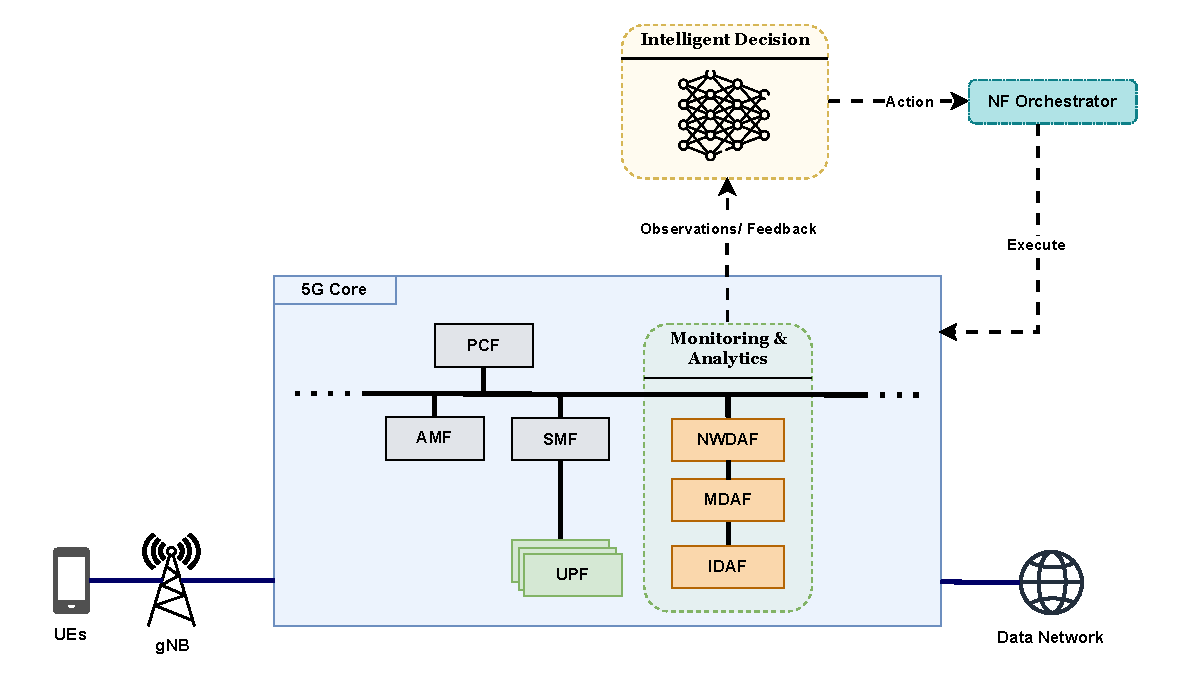
\includegraphics[width=.9\textwidth]{closed_loop.pdf}
\caption{Target online closed-loop UPF orchestration architecture. The present paper validates the decision logic offline in a measurement-grounded digital twin before any live deployment.}
\label{fig:closedloop}
\end{figure}

\subsection{5GC User-Plane Model}

The 5GC domain includes the control-plane functions and the user-plane function. In the proposed architecture, the UPF is the controlled element subject to orchestration. Control-plane functions are treated as external to the optimization loop; they provide service context and support UPF endpoint configuration, but they are not decision variables in our model.

\subsection{UPF Configuration Space}
\label{subsec:cfgspace}

We consider two UPF realization classes with different performance--energy characteristics:

\textbf{DPDK-based UPF} is a kernel-bypass, polling-driven packet-processing pipeline designed for high throughput and low latency.

\textbf{User-space UPF} is a general-purpose software UPF deployed as containerized instances that can be scaled horizontally.

We model the deployment as a discrete configuration that captures both the realization mode and its horizontal scale. Let $\mathcal{M}$ be the set of supported UPF modes. In this work, $\mathcal{M}=\{\mathrm{DPDK},\mathrm{USR}\}$, where $\mathrm{DPDK}$ denotes a DPDK-based dataplane and $\mathrm{USR}$ denotes a cloud-native user-space dataplane. For each mode $m\in\mathcal{M}$, we define a finite set of admissible instance counts $\mathcal{K}_m \subset \mathbb{N}$. A configuration at slot $t$ is represented as
\begin{equation}
    c_t = (m_t,k_t), \qquad m_t\in\mathcal{M},\; k_t\in\mathcal{K}_{m_t},
\end{equation}
and the overall configuration space is
\begin{equation}
    \mathcal{C}=\bigcup_{m\in\mathcal{M}}\{m\}\times\mathcal{K}_m.
\end{equation}

The concrete mode set $\mathcal{M}$, admissible instance counts $\mathcal{K}_m$, and resulting configuration space $\mathcal{C}$ used in the evaluation are specified in Section~\ref{testbed_hw}.

\subsection{Monitoring and Analytics}
\label{subsec:monitoring}

Monitoring and analytics operate on a slotted time base. Time is divided into control slots of duration $\Delta$, indexed by $t\in\mathbb{N}$. During each slot, raw telemetry is collected from network functions and the hosting infrastructure, then aggregated into slot-level indicators aligned to the slot timestamp. We collect these indicators in an observation vector $x_t$, which is used by the decision module.

The indicators fall into three groups. Traffic indicators summarize the offered load during the slot. QoS indicators summarize service compliance during the slot. Resource and energy indicators summarize the footprint of the active deployment. In the remainder of the paper, the energy-related signal is represented through slot-averaged UPF-attributed power $P_t$ on the hosting node; slot energy is then derived as $E_t=P_t\Delta$ when needed. The emphasis on attributed power is important: the quantities used in the controller and evaluation are process-level estimates attributed to the UPF processes rather than full server power measurements.

The required indicators can be obtained through analytics functions supported by the 5G SBA. Network-facing analytics can be provided through the Network Data Analytics Function (NWDAF), which collects and exposes network-level indicators to consumers~\cite{bolla10465014}. Infrastructure-facing indicators, including resource usage and power-related metrics, can be exposed through a Management Data Analytics Function (MDAF). In energy-oriented realizations, the MDAF can retrieve such KPIs from cloud-native infrastructure resources through the metrics exposed by an infrastructure data collection function (IDAF) rather than by directly accessing the infrastructure~\cite{AKBARI2025111487}.

\subsection{Orchestration and Actuation Guard}
\label{subsec:actuation}

At each control slot, the orchestration layer receives a configuration command and translates it into an actuation on the UPF deployment. Actuation updates the active realization mode and, when applicable, the number of active instances. The resulting deployed state for slot $t$ is represented by the executed configuration $c_t\in\mathcal{C}$.

To prevent rapid oscillations, configuration changes are regulated by an explicit cooldown guard. Let $u_t$ be the number of elapsed control slots since the last executed reconfiguration, and let $I_c$ be the cooldown length in slots. Given a requested configuration command $a_t\in\mathcal{C}$, the executed configuration is obtained as
\begin{equation}
    c_t =
    \begin{cases}
        a_t, & \text{if } u_t \ge I_c,\\
        c_{t-1}, & \text{otherwise}.
    \end{cases}
    \label{eq:cooldown_guard}
\end{equation}
The cooldown state is reset whenever a reconfiguration is executed and increases by one slot otherwise. This guard is applied uniformly across all controllers considered in the paper. Embedding it in the environment transition function makes the minimum dwell time part of the control problem itself rather than a post-processing rule.

\subsection{Decision Interface}
\label{subsec:decision_interface}

At slot $t$, the decision module receives the observation vector $x_t$ together with the current deployment context and outputs a configuration command $a_t\in\mathcal{C}$. The orchestration layer enforces the actuation guard in Section~\ref{subsec:actuation} to obtain the executed configuration $c_t\in\mathcal{C}$, which determines the UPF deployment during slot $t$ and influences the observations collected at subsequent decision boundaries.

\section{RL-Based Orchestration Framework}
\label{method}

This section formalizes the decision module as a sequential decision-making problem and describes the learning environment used in the evaluation. The formulation follows the same control period $\Delta$ and the guarded actuation semantics introduced in Section~\ref{subsec:decision_interface} and Section~\ref{subsec:actuation}. In the present study, all controller learning and comparison are carried out offline in the digital twin rather than by executing the controller live on the physical testbed.

\subsection{Decision Process Formulation}
\label{subsec:mdp_formulation}

We formulate the closed-loop interaction as a Markov decision process defined at decision epochs indexed by $t\in\mathbb{N}$. At each epoch, the agent observes $x_t$ and issues a configuration command $a_t\in\mathcal{C}$. The orchestration layer enforces the cooldown guard and determines the executed configuration. A reward $r_t$ is then computed from the power and QoS outcomes observed over the subsequent control interval, and the next observation $x_{t+1}$ becomes available at the following decision boundary.

The learning objective is to find a policy $\pi_\theta$ that maximizes the expected discounted return
\begin{equation}
J(\pi_\theta)=\mathbb{E}_{\pi_\theta}\!\left[\sum_{t=0}^{T-1}\gamma^t r_t\right],
\label{eq:return}
\end{equation}
where $\gamma\in(0,1]$ is the discount factor and $T$ is the episode length.

In practice, the agent observes aggregated indicators rather than the full latent network state. The problem is therefore only partially observed from the controller's perspective. We address this by considering multiple observation constructions, including finite traffic history, optional forecast inputs, and recurrent policies. The concrete observation schema used in each experiment is specified in Section~\ref{testbed}.

\subsection{Digital-Twin Environment and Outcome Signals}
\label{subsec:digital_twin}

Direct exploration on an operational 5GC user plane is impractical because disruptive reconfigurations carry real service cost. We therefore employ a data-driven digital twin that provides a controlled environment for learning and for fair comparison across controllers. The twin emulates the outcome of applying an executed configuration $c_t$ under the traffic conditions of the corresponding control interval.

For each decision epoch $t$, the twin returns two outcome signals. The first is the UPF-attributed power draw $P_t$ under $c_t$, represented as the interval-averaged attributed power over the control period. The second is a QoS outcome $Q_t$ that summarizes service compliance for the same period through a scalar performance indicator. These signals are computed with the same procedure for all evaluated controllers and are used to construct the reward in Section~\ref{subsec:reward} and the evaluation metrics in Section~\ref{result}.

\subsection{Observation Space and Schemas}
\label{subsec:obs_space}

The agent input $x_t$ is constructed from the indicator families introduced in Section~\ref{subsec:monitoring}. It summarizes traffic conditions, service outcomes, and the energy-related signal observed at the decision boundary. In addition, $x_t$ includes the minimal deployment context required by the actuation semantics, namely the previously executed configuration and the cooldown status.

We evaluate four observation schemas that differ only in how traffic context is provided:
\begin{itemize}
    \item \textbf{Instantaneous:} $x_t$ includes the current traffic load $\rho_t$ together with the current QoS and energy indicators and the deployment context.
    \item \textbf{History-augmented:} $x_t$ augments the instantaneous schema with a window of past traffic loads $\rho_{t-W+1:t}$ of length $W$.
    \item \textbf{Forecast-augmented:} $x_t$ augments the instantaneous schema with a forecast vector $\hat{\rho}_{t+1:t+H}$ of horizon $H$.
    \item \textbf{Hybrid:} $x_t$ includes both the history window $\rho_{t-W+1:t}$ and the forecast vector $\hat{\rho}_{t+1:t+H}$ in addition to the instantaneous indicators.
\end{itemize}

These schemas address the fact that the controller observes aggregated indicators rather than the full latent network state. For each experiment, the schema and its parameters $(W,H)$ are fixed and kept identical across the compared controllers.

\subsection{Action Space and Configuration Encoding}

\label{subsec:action_space}

The decision module selects configuration commands from the configuration space $\mathcal{C}$ defined in Section~\ref{subsec:cfgspace}. In the implementation, commands are represented as discrete action indices. A one-to-one mapping is used between the finite set of admissible configurations and the discrete action set, so that each action index corresponds to exactly one configuration command.

\subsection{Reward Design}
\label{subsec:reward}

The reward balances energy efficiency, QoS compliance, and orchestration stability. Energy efficiency is captured through the specific energy consumption
\begin{equation}
\mathrm{SEC}_t=\frac{P_t}{\max(\rho_t,\epsilon)},
\label{eq:sec}
\end{equation}
where $P_t$ is the interval-averaged attributed power returned by the digital twin, $\rho_t$ is the offered load over the same interval, and $\epsilon$ is a small constant used for numerical stability.

QoS compliance is enforced through a soft penalty based on the scalar compliance indicator $Q_t$ and a target threshold $\tau$:
\begin{equation}
\mathcal{L}^{\mathrm{QoS}}_t=\lambda_{\mathrm{QoS}}\max(0,\tau-Q_t),
\label{eq:qos_penalty}
\end{equation}
where $\lambda_{\mathrm{QoS}}$ controls the penalty strength.

Orchestration stability is encouraged by penalizing executed reconfigurations. Let $c_{t-1}$ and $c_t$ be the executed configurations before and after the actuation guard. A switching penalty is applied when the realization mode changes between $c_{t-1}$ and $c_t$, and a scaling penalty is applied when the realization mode is unchanged but the instance count changes. These contributions are combined into a single orchestration cost $\mathcal{L}^{\mathrm{ORCH}}_t$.

The resulting reward is
\begin{equation}
r_t=-\alpha\,\mathrm{SEC}_t-\mathcal{L}^{\mathrm{QoS}}_t-\mathcal{L}^{\mathrm{ORCH}}_t,
\label{eq:reward}
\end{equation}
where $\alpha$ scales the SEC contribution. Using SEC rather than raw power in the energy term discourages trivially low-power but low-throughput operating points. The asymmetric weighting of switching and scaling penalties encourages the learned controller to prefer lower-cost horizontal scaling operations over more disruptive mode changes when possible. The weights and cost parameters used in the experiments are reported in Section~\ref{testbed}.

\subsection{Learning Algorithm}
\label{subsec:rl_algo}

The policy $\pi_\theta$ is learned using Proximal Policy Optimization (PPO), an on-policy actor--critic method that supports discrete action spaces and delayed-consequence control. PPO learns a stochastic policy over configuration commands together with a value function that estimates the expected return. Training optimizes the objective in~\eqref{eq:return} from trajectories generated under the guarded actuation semantics defined in Section~\ref{subsec:actuation}.

We consider two PPO parameterizations. In the feed-forward variant, temporal context is supplied through the observation construction. In the recurrent variant, the policy includes an internal memory state that integrates information across decision epochs. We do not claim PPO is the only suitable method for a small configuration space; rather, it provides a consistent policy-gradient baseline for a constrained sequential-control setting and a natural path toward larger future configuration spaces. The specific variant and training hyperparameters used in each experiment are reported in Section~\ref{testbed}.



\subsection{Baseline Controllers}
\label{subsec:baselines}

We compare the PPO-based controller against static and rule-based baselines. These baselines are part of the controller methodology rather than of the workload setup, so we define them here before introducing the evaluation protocol. All controllers operate on the same configuration space $\mathcal{C}$ and, unless explicitly stated otherwise, are evaluated through the same digital twin described in Section~\ref{subsec:twin_construction}.

\textbf{Static provisioning.} We include static baselines in which the UPF configuration is kept constant over the full evaluation horizon. In the reported results, we consider static DPDK and static USR($k=1$), which provide references for the case where no dynamic orchestration is performed.

\textbf{Rule-based threshold selector.} This baseline follows threshold logic derived from the profiling curves. Offline, we compare the attributed-power and QoS profiling curves of the admissible configurations and identify the throughput regions in which each configuration is preferred under the target QoS threshold. Online, the controller maps the one-step-ahead traffic forecast to the corresponding configuration region and issues the associated command. To reduce oscillations around region boundaries, it applies a dead-band around each threshold and the same cooldown guard used by the PPO controllers.

\textbf{Offline-optimal reference.} We additionally compute a non-causal offline-optimal reference using exact finite-horizon dynamic programming over the deterministic digital twin. This planner has access to the full test-sequence load trajectory and uses the same configuration space, cooldown semantics, reconfiguration costs, and discounted cumulative reward objective as PPO, with $\gamma=0.995$. It is therefore not a deployable controller, but it provides an upper bound with respect to the modeled control problem and quantifies how much of the available performance gap is captured by the causal controllers.


\section{Physical Testbed and Data Collection}

\label{testbed_hw}

This section describes the physical infrastructure used to characterize UPF behavior, the profiling campaign that produced the data used to fit the profiling models, and the measurement assumptions that underpin the digital twin used in the evaluation.

\subsection{Infrastructure and UPF Configurations}
\label{subsec:hw_infra}

The testbed consists of a commodity server running both UPF instances and the traffic generator on the same physical host, with power measurements obtained at the process level. The DPDK-based UPF is realized using the SD-Core user plane, which provides a kernel-bypass, polling-driven packet-processing pipeline. The cloud-native UPF is realized using the Open Air Interface (OAI) UPF, hereafter referred to as the USR UPF, and is deployed as containerized instances managed by a Kubernetes orchestrator that supports horizontal scaling through replica control. Figure~\ref{fig:testbed_system} should therefore be read as the profiling and measurement setup used to characterize UPF behavior; the PPO controller is not trained or evaluated in live closed loop on this physical setup in the current paper.

\begin{figure}
\centering
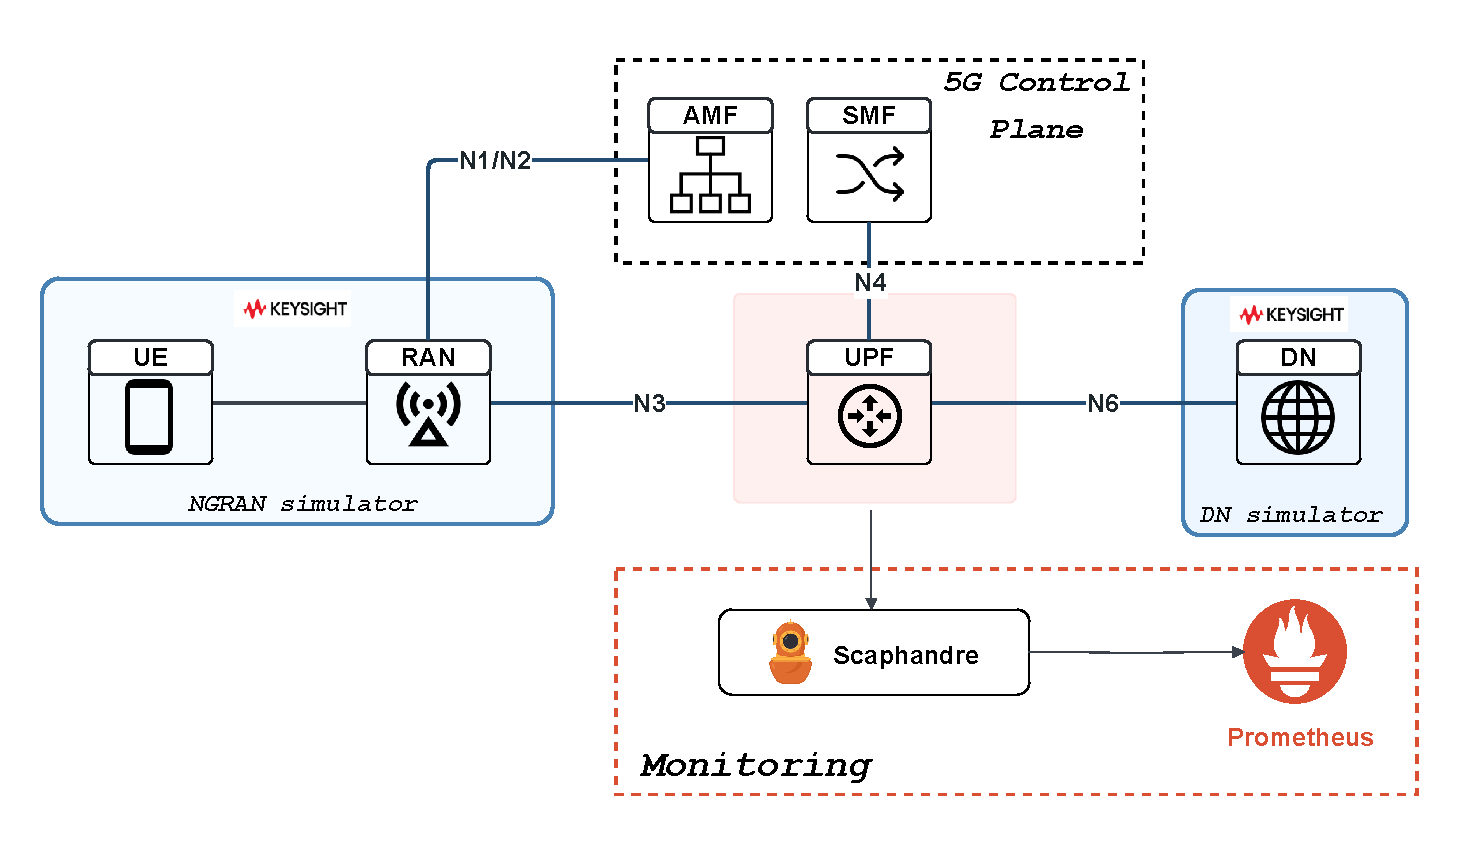
\includegraphics[width=.75\textwidth]{2_3_system.pdf}
\caption{Physical testbed architecture used for UPF profiling and metric collection. The Keysight LoadCore platform simulates UE/RAN (N3) and data-network (N6) endpoints. The 5G control plane (AMF, SMF) manages sessions via N4. Scaphandre monitors power attributed to the UPF processes via RAPL-derived estimates and exports metrics to Prometheus.}
\label{fig:testbed_system}
\end{figure}

The concrete configuration space instantiated on this testbed is $\mathcal{M}=\{\mathrm{DPDK},\mathrm{USR}\}$ with $\mathcal{K}_{\mathrm{DPDK}}=\{1\}$ and $\mathcal{K}_{\mathrm{USR}}=\{1,2\}$, yielding a total of $|\mathcal{C}|=3$ admissible configurations: one DPDK instance, one USR instance, and two USR instances. A single DPDK instance is sufficient to serve the full load range considered in the evaluation without performance degradation, so no horizontal scaling is defined for that mode. The USR mode supports up to two instances, reflecting the capacity limit of a single USR instance under the traffic conditions of this work.

Power consumption is measured with Scaphandre, an open-source monitoring tool that estimates per-process energy draw from hardware counters exposed by the RAPL interface. Infrastructure-level metrics including CPU utilization and memory are collected via Prometheus. Traffic is generated using stateless UDP flows with a fixed packet size of 1250 bytes, produced by Keysight LoadCore.

Because the power signal is process-attributed rather than a full server power trace, the watt and watt-hour quantities reported in this paper should be interpreted as \emph{UPF-attributed estimates} used consistently for profiling, reward construction, and controller comparison within this testbed.

\subsection{Profiling Campaign}
\label{subsec:profiling}

Figure~\ref{fig:offline_pipeline} illustrates the three-stage offline workflow used in this paper. The profiling module characterizes the two UPF realizations on the physical testbed and produces the profiling-model repository, the forecasting module prepares the traffic workload and trains the one-step-ahead predictor, and the digital-twin/RL module assembles these components into a simulation environment in which PPO is trained and evaluated offline. The bottom ``Deploy to online closed-loop controller'' box represents the intended later deployment target of the trained artifacts and is not part of the experimental validation reported here.

\begin{figure}
\centering
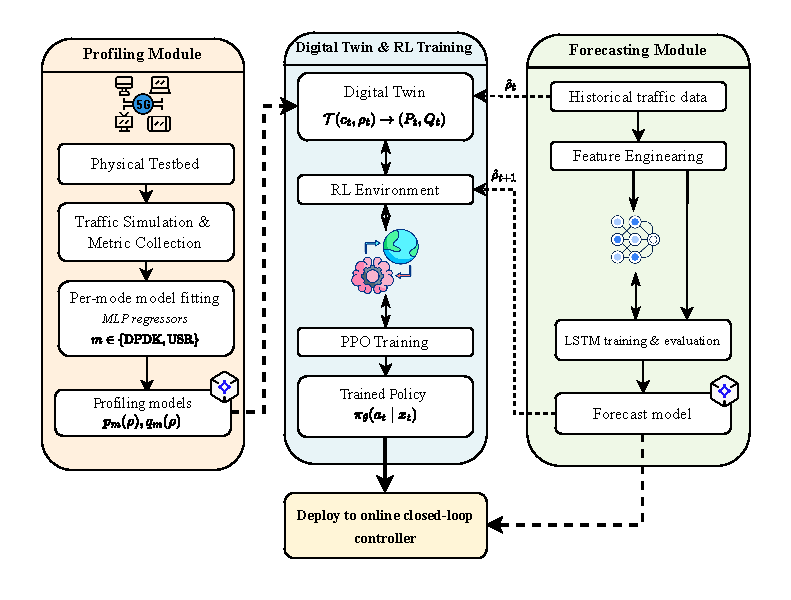
\includegraphics[width=.9\textwidth]{offline_pipeline.pdf}
\caption{Offline workflow used in this paper for data collection, profiling-model fitting, forecasting, and PPO policy learning. The trained policy $\pi_\theta$, forecast model, and profiling models $(p_m,q_m)$ are produced offline; the final deployment box indicates intended future use in the online control loop and is not part of the present evaluation.}
\label{fig:offline_pipeline}
\end{figure}

The profiling models are trained from a profiling dataset collected by subjecting each UPF configuration to a sweep of 22 offered-load levels spanning the range from \SI{0.01}{Mbps} to \SI{5}{Gbps}. The load levels are defined by the packet-rate sequence at the fixed packet size. Each load level is sustained for a fixed measurement window and repeated across multiple runs to capture measurement variability. The traffic direction is downlink only, consistent with the traffic model adopted for the evaluation workload.

QoS is assessed against the service requirements of 5QI=9 (video buffered streaming, non-GBR) as standardized in 3GPP TS~23.501~\cite{3gpp23501}. The corresponding thresholds are a packet delay budget $D_{\max}=300$~ms, a jitter bound $J_{\max}=100$~ms, and a packet error rate $L_{\max}=10^{-6}$. Each KPI is mapped to a bounded score, and the final scalar QoS-compliance signal used by the twin is defined in Section~\ref{subsec:twin_construction}.

Figure~\ref{fig:power_model} shows the measured attributed-power distributions and fitted profiling curves for both UPF realizations as a function of offered throughput. In this testbed, the DPDK-based UPF exhibits a nearly load-independent attributed-power profile at approximately 0.75~W, while the USR attributed power increases monotonically from near zero at idle to approximately 3.2~W at saturation. Figure~\ref{fig:qos_model} shows the corresponding QoS-compliance scores. DPDK maintains near-perfect compliance ($Q\approx0.96$) across the full load range. The USR sustains compliance above $\tau=0.9$ up to approximately 400~Mbps per instance, beyond which the score degrades sharply. These profiles motivate the orchestration problem by showing that the two realizations expose different attributed-power and QoS behavior across load.

\begin{figure}
\centering
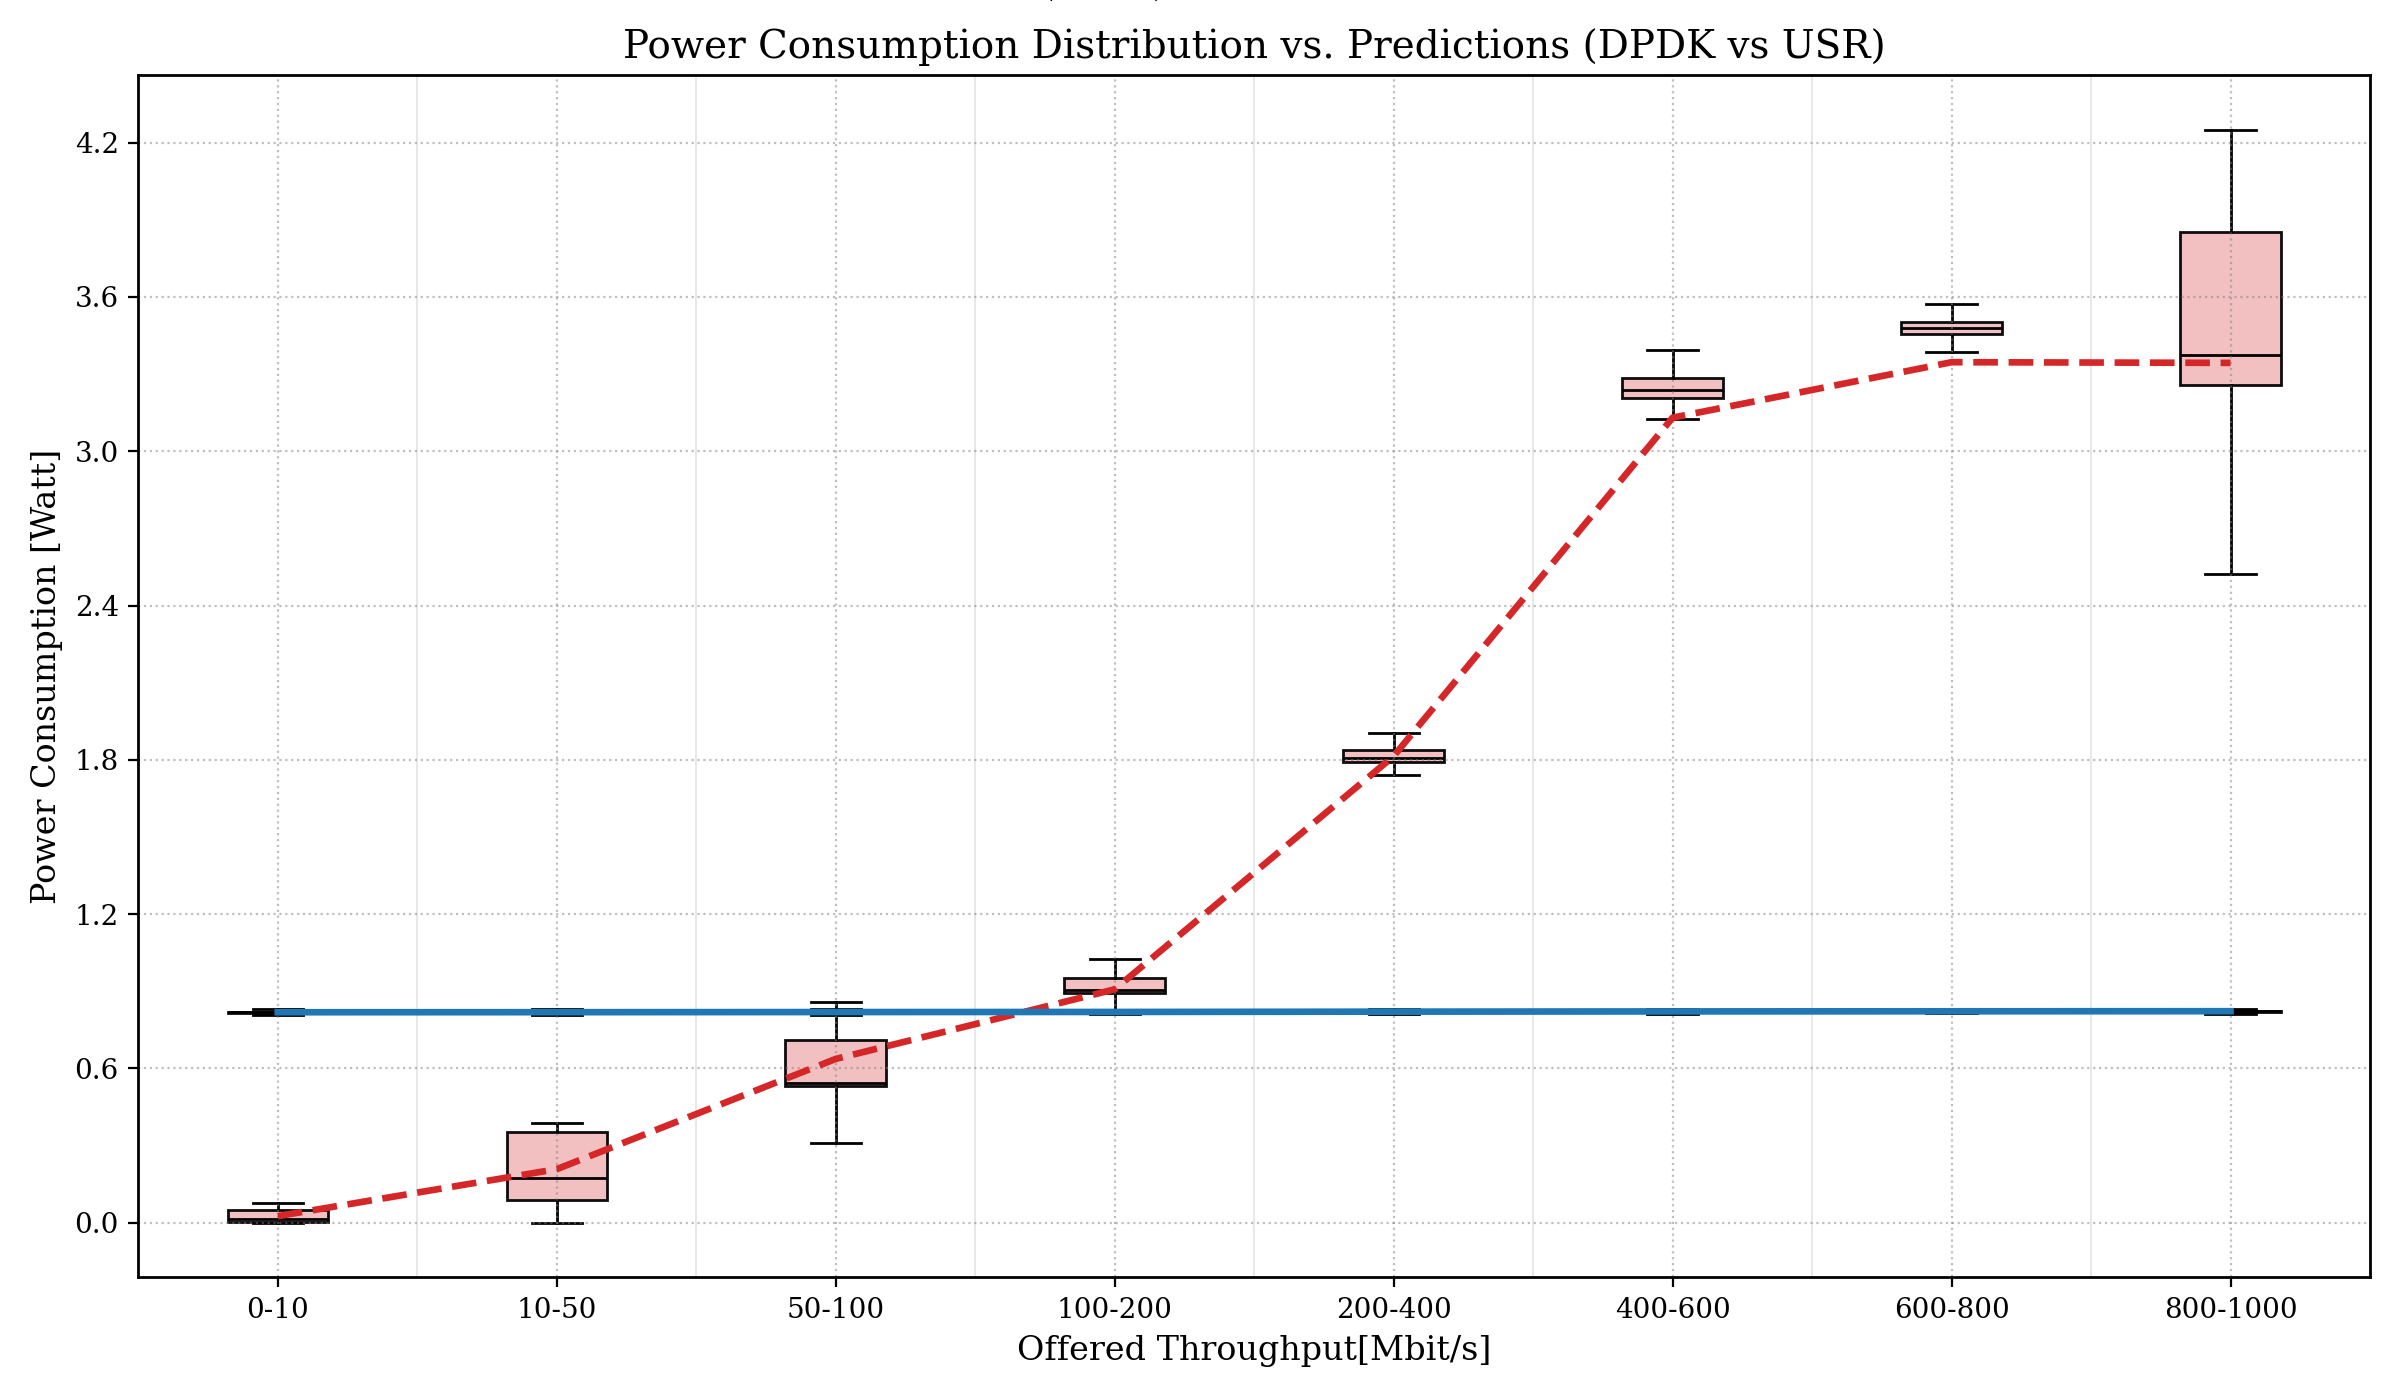
\includegraphics[width=.75\textwidth]{power_model_learned_curves.png}
\caption{Process-attributed power-consumption distributions and MLP profiling-model predictions for the DPDK (blue, solid) and USR (red, dashed) realizations as a function of offered throughput. Box plots show empirical variability across profiling runs.}
\label{fig:power_model}
\end{figure}

\begin{figure}
\centering
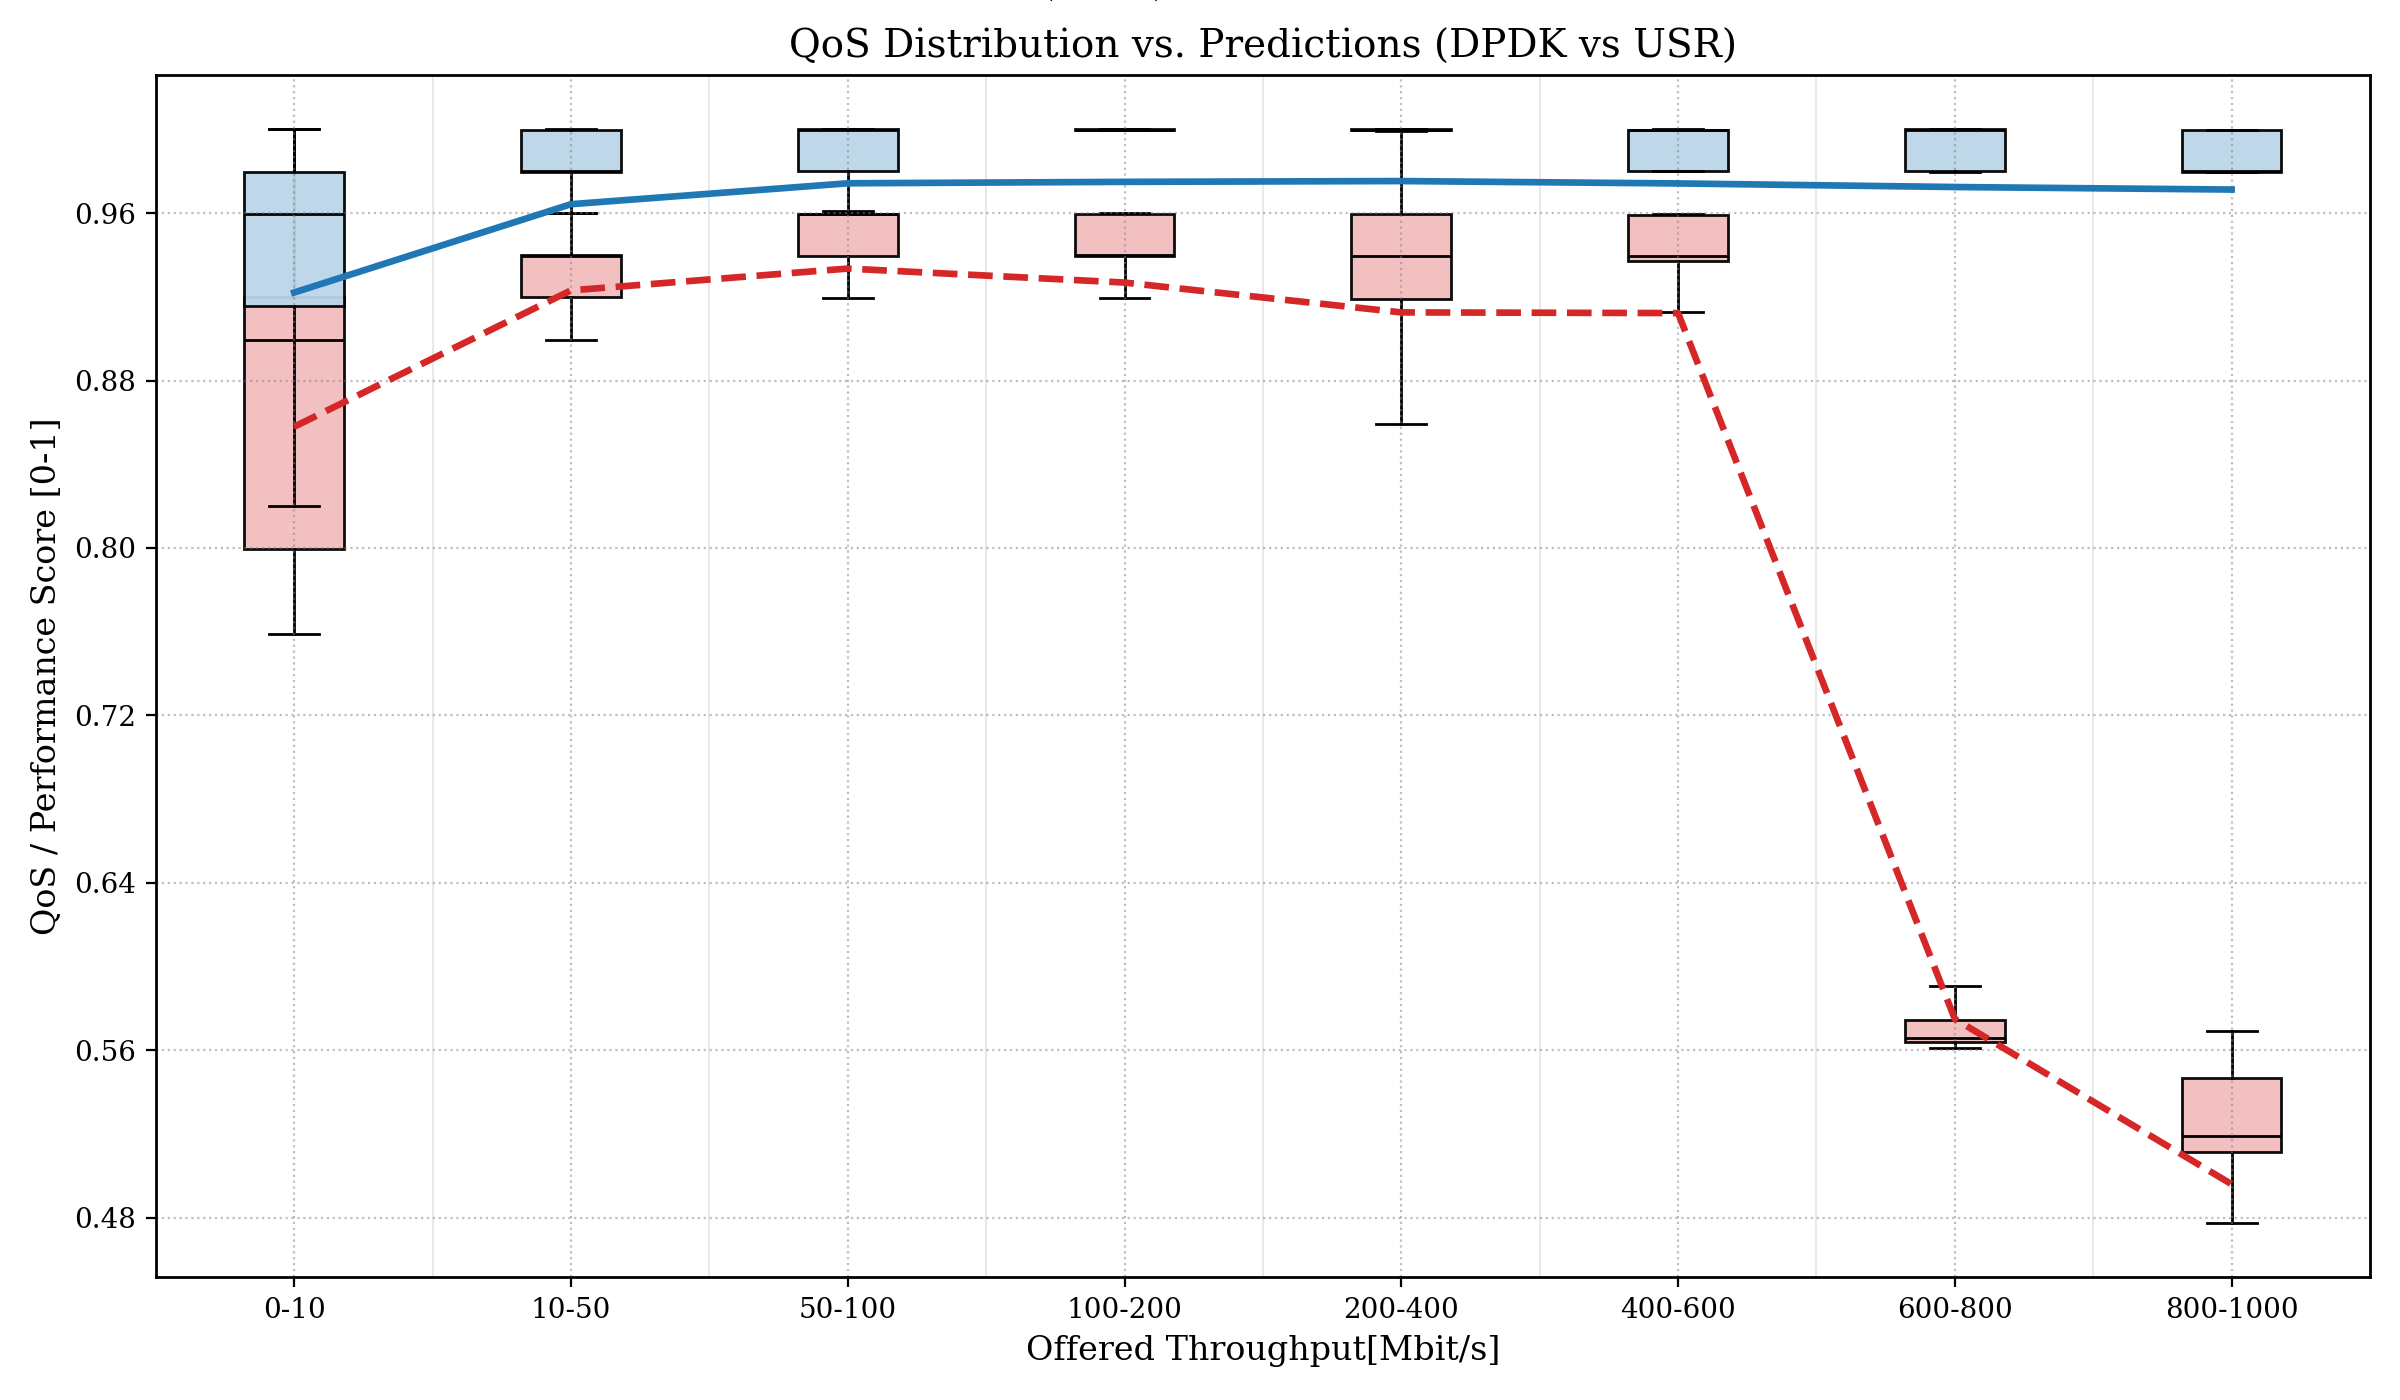
\includegraphics[width=.75\textwidth]{performance_model_learned_curves.png}
\caption{QoS-compliance score distributions and MLP profiling-model predictions for both UPF realizations. The dashed line marks the compliance target $\tau=0.9$. The USR score degrades sharply above approximately 400~Mbps per instance.}
\label{fig:qos_model}
\end{figure}

\subsection{Profiling Models and Digital-Twin Construction}
\label{subsec:twin_construction}

The evaluation relies on a data-driven digital twin that emulates the user-plane outcomes of applying a configuration $c_t=(m_t,k_t)\in\mathcal{C}$ under load $\rho_t$. No controller is executed live on the physical testbed in this study; instead, all results are obtained by replaying the workload through this common profiling-model-based environment. The twin provides two outcome signals for each control interval:
\begin{itemize}
    \item the interval-averaged UPF-attributed power draw $P_t$; and
    \item a scalar QoS-compliance score $Q_t$ for the same interval.
\end{itemize}

Both signals are obtained from profiling models trained offline on the profiling data. For each UPF realization mode $m\in\mathcal{M}$, we fit two MLP regressors, one for attributed power and one for QoS compliance, using per-instance offered load as input. Denoting these profiling models by $p_m(\rho)$ and $q_m(\rho)$, the twin evaluates
\begin{equation}
(P_t,Q_t)=\mathcal{T}(c_t,\rho_t),
\end{equation}
where $\mathcal{T}(\cdot)$ applies the mode-specific profiling models and accounts for horizontal scaling when $k_t>1$.

The QoS outcome is represented through a scalar compliance score $Q_t$ obtained by aggregating multiple KPIs observed over the control interval. Let $S^{\mathrm{lat}}_t$, $S^{\mathrm{jit}}_t$, and $S^{\mathrm{loss}}_t$ denote bounded component scores associated with delay, jitter, and packet loss, respectively. Each component is mapped to a normalized score through a bounded scoring function with service thresholds $(D_{\max},J_{\max},L_{\max})$. The resulting QoS score is computed as
\begin{equation}
Q_t = w_{\mathrm{lat}} S^{\mathrm{lat}}_t + w_{\mathrm{jit}} S^{\mathrm{jit}}_t + w_{\mathrm{loss}} S^{\mathrm{loss}}_t,
\label{eq:qos_weighted}
\end{equation}
with non-negative weights $\sum_i w_i = 1$. In the evaluation, QoS components are weighted as $(w_{\mathrm{lat}}, w_{\mathrm{jit}}, w_{\mathrm{loss}}) = (0.40, 0.40, 0.20)$, reflecting equal emphasis on delay and jitter compliance for buffered video-streaming traffic under 5QI=9 and a lower weight on packet loss.

For multi-instance configurations, we assume that traffic is distributed across the $k_t$ active instances by a load-balancing mechanism that yields an approximately even split. Accordingly, the per-instance offered load is approximated as $\rho_t/k_t$. Under the balanced-split assumption, the twin computes
\begin{equation}
P_t = k_t\, p_{m_t}\!\left(\frac{\rho_t}{k_t}\right),
\label{eq:power_aggregate}
\end{equation}
and derives the interval QoS-compliance score as
\begin{equation}
Q_t = q_{m_t}\!\left(\frac{\rho_t}{k_t}\right).
\label{eq:qos_aggregate}
\end{equation}

For each mode and target, a small MLP regressor is trained on an 80/20 held-out split of the profiling data, using log-transformed offered throughput as the sole input feature. Model complexity (depth, regularization) is chosen per target to match the difficulty of the regression; the DPDK attributed-power model is shallow because the target is nearly constant, whereas the USR models use deeper architectures with batch normalization and dropout to capture the steeper load--response curves. Table~\ref{tab:profiling_acc} reports held-out accuracy for the four fitted profiling models.

\begin{table}[width=.9\linewidth,cols=4,pos=h]
\centering
\caption{Held-out accuracy of the profiling models used by the digital twin. Metrics are computed on the 20\% held-out split.}
\label{tab:profiling_acc}
\begin{tabular}{l l c c}
\hline
Mode & Target & RMSE & $R^2$ \\
\hline
DPDK & QoS score        & 0.0847 & 0.153 \\
DPDK & Attributed power & 0.0039 & 0.239 \\
USR  & QoS score        & 0.0785 & 0.907 \\
USR  & Attributed power & 0.3038 & 0.960 \\
\hline
\end{tabular}
\end{table}

The profiling models introduce a controlled approximation: the twin captures the mean load--response relationship but does not reproduce measurement noise or transient effects. This provides a deterministic evaluation environment that removes one source of variance from the controller comparison, while the profiling variability shown in Figures~\ref{fig:power_model} and~\ref{fig:qos_model} gives a qualitative indication of the uncertainty present in the underlying system.

\section{Experimental Setup}
\label{testbed}

This section describes the workload data and evaluation protocol used to assess the controllers introduced in Section~\ref{method}. Unless explicitly stated otherwise, all controller comparisons in this section are performed offline in the same digital twin under replayed workload conditions.

\subsection{Workload Traces and Time Base}
\label{subsec:workload}

The primary evaluation workload is derived from the NetMob 2023 dataset~\cite{netmob2023}, which provides spatially disaggregated, service-level mobile traffic demand across French cities. We use the downlink traffic volume attributed to Netflix streaming in the city of Lyon, aggregated across spatial units to obtain a single city-level time series. We refer to this as the \emph{Main trace}. The raw traffic is normalized and rescaled so that the maximum offered load does not exceed 400~Mbps, keeping the peak demand within the profiled operating range and within the single-instance USR capacity boundary identified during profiling. This scaling avoids extrapolating the profiling models beyond the measurement envelope while preserving a workload that exercises both realization-mode selection and USR scale selection.

To assess cross-trace generalization, we derive a second workload from the same NetMob 2023 dataset using the downlink traffic volume attributed to YouTube streaming in the same city and time period. We refer to this as the \emph{YouTube trace}. The same normalization and rescaling procedure is applied. Because the YouTube service class exhibits a different diurnal pattern and load distribution compared to Netflix, this trace provides an independent check of whether policies trained on the Main trace transfer to an unseen traffic profile without retraining.

The Main trace spans the period from 2019-04-01 00:00 to 2019-05-05 23:45, yielding $N=3{,}359$ control slots at the 15-minute control period $\Delta=15$~min. The dataset is split chronologically at a 75/25 ratio, giving $N_{\mathrm{tr}}=2{,}519$ training slots ($\approx$26~days) and $N_{\mathrm{te}}=840$ test slots ($\approx$9~days). No shuffling is applied in order to preserve temporal structure and avoid leakage across time. The YouTube trace follows the same temporal extent and split ratio.

One-step-ahead traffic forecasts $\hat{\rho}_{t+1}$, used by the forecast-augmented and hybrid observation schemas, are produced by an LSTM-based sequence model trained on a temporal split of the Main traffic series (no shuffling). The predictor uses calendar features and a 96-sample input window. Table~\ref{tab:forecast_acc} reports its held-out accuracy in project load-scaled traffic units.

\begin{table}[width=.9\linewidth,cols=4,pos=h]
\centering
\caption{Held-out accuracy of the traffic predictor used by the forecast-augmented and hybrid observation schemas.}
\label{tab:forecast_acc}
\begin{tabular}{l c c c}
\hline
Predictor & Horizon & RMSE & $R^2$ \\
\hline
LSTM-based traffic predictor  & \(t{+}1\) & 19.12 & 0.898 \\
\hline
\end{tabular}
\end{table}

\subsection{Key Configuration Parameters}

\label{subsec:key_params}

Table~\ref{tab:testbed_params} summarizes the main parameters used in the experimental campaign, including the cooldown length, reward weights, and PPO hyperparameters.

\begin{table}[width=.9\linewidth,cols=2,pos=h]
\centering
\caption{Main experimental parameters used in the evaluation.}
\label{tab:testbed_params}
\begin{tabular}{l c}
\hline
Parameter & Value \\
\hline
Control period & $\Delta = 15$~min \\
Cooldown length & $I_c=4$ \\
QoS target threshold & $\tau=0.9$ \\
SEC scaling in reward & $\alpha=100$ \\
QoS penalty weight & $\lambda_{\mathrm{QoS}}=30$ \\
Type switch cost & $0.5$ \\
Scale-up cost per instance & $0.2$ \\
Scale-down cost per instance & $0.05$ \\
Discount factor & $\gamma=0.995$ \\
PPO rollout steps & $n_{\mathrm{steps}}=1024$ \\
Batch size & $64$ \\
Epochs per update & $10$ \\
Learning rate & $10^{-4}$ \\
Entropy coefficient & $0.15$ \\
Clip range & $0.2$ \\
GAE parameter & $0.9$ \\
Total training steps & $3\times 10^{5}$ \\
Train/test split ratio & $0.75 / 0.25$ \\
% Parallel environments & $4$ \\
\hline
\end{tabular}
\end{table}

All PPO training is performed on a single CPU without GPU acceleration. At the target budget of $3\times10^5$ timesteps, training one feed-forward PPO seed takes approximately 7.4~minutes (443~s wall-clock), while one recurrent PPO seed takes approximately 11.6~minutes (693~s). The five-seed robustness runs reported in Section~\ref{subsec:seed_robustness} require about 37~minutes total for the feed-forward variant and about 58~minutes for the recurrent variant.

\section{Results \& Analysis}
\label{result}

This section reports the performance of the controllers introduced in Section~\ref{method} under the experimental protocol described in Section~\ref{testbed}. All results are computed on the held-out test split, in offline replay through the digital twin, and under the same actuation guard from Section~\ref{subsec:actuation}. Unless otherwise stated, comparisons are performed on the executed configuration sequence $\{c_t\}$ and the corresponding twin outcomes $\{(P_t,Q_t)\}$.

\subsection{Evaluation Metrics}
\label{subsec:metrics}

We quantify energy efficiency, QoS compliance, and orchestration behavior using three metric groups.

Energy is measured by integrating the interval-averaged attributed-power trace over the evaluation horizon:
\begin{equation}
E_{\mathrm{tot}}=\sum_{t=0}^{N_{\mathrm{te}}-1} P_t \Delta.
\label{eq:total_energy}
\end{equation}
In addition, we report the average specific energy consumption
\begin{equation}
\overline{\mathrm{SEC}}=\frac{1}{N_{\mathrm{te}}}\sum_{t=0}^{N_{\mathrm{te}}-1}\frac{P_t}{\max(\rho_t,\epsilon)}.
\label{eq:avg_sec}
\end{equation}

QoS compliance is summarized through the scalar outcome $Q_t$ produced by the digital twin. Given the compliance target $\tau$, we report the violation rate
\begin{equation}
v=\frac{1}{N_{\mathrm{te}}}\sum_{t=0}^{N_{\mathrm{te}}-1}\mathbb{I}\{Q_t<\tau\},
\label{eq:violation_rate}
\end{equation}
and the average compliance indicator $\overline{Q}=\frac{1}{N_{\mathrm{te}}}\sum_t Q_t$.

Orchestration behavior is characterized by disaggregating reconfigurations into two event types. Type-switch events, counted as
\begin{equation}
n_{\mathrm{sw}}=\sum_{t=1}^{N_{\mathrm{te}}-1}\mathbb{I}\{m_t\neq m_{t-1}\},
\label{eq:nsw}
\end{equation}
capture mode changes between DPDK and USR. Horizontal scaling events, counted as
\begin{equation}
n_{\mathrm{sc}}=\sum_{t=1}^{N_{\mathrm{te}}-1}\mathbb{I}\{m_t= m_{t-1},\, k_t\neq k_{t-1}\},
\label{eq:nsc}
\end{equation}
capture changes in the number of active USR instances under a fixed mode. We also report $n_{\mathrm{bl}}$, the number of change requests absorbed by the cooldown guard without actuation, and dwell-time statistics defined as the empirical distribution of consecutive intervals spent in the same executed configuration.

\subsection{Overall Comparison Across Controllers}
\label{subsec:overall}

Table~\ref{tab:overall_results} provides a consolidated comparison of the controllers on energy, QoS, and stability metrics. Because the static and rule-based baselines are deterministic, their results are single values; the PPO rows report mean $\pm$ standard deviation over five independently trained seeds on the main held-out evaluation split. The rule-based controller uses the same configuration space $\mathcal{C}$ and the same cooldown guard, so differences are attributable to decision logic rather than to actuation semantics.

\begin{table}[width=.9\linewidth,cols=7,pos=h]
\centering
\caption{Overall results on the main held-out evaluation split. Lower is better for $E_{\mathrm{tot}}$, $\overline{\mathrm{SEC}}$, and $v$. $n_{\mathrm{sw}}$ counts type-switch events (DPDK$\leftrightarrow$USR); $n_{\mathrm{sc}}$ counts horizontal scaling events (USR instance-count changes); $n_{\mathrm{bl}}$ counts change requests blocked by the cooldown guard. $E_{\mathrm{tot}}$ is in Wh and $\overline{\mathrm{SEC}}$ in Wh/Mbit. PPO rows report mean $\pm$ standard deviation over five seeds.}
\label{tab:overall_results}
\small
\resizebox{\columnwidth}{!}{%
\begin{tabular}{l c c c c c c}
\hline
Controller & $E_{\mathrm{tot}}$ & $\overline{\mathrm{SEC}}$ & $v$ & $n_{\mathrm{sw}}$ & $n_{\mathrm{sc}}$ & $n_{\mathrm{bl}}$ \\
\hline
Offline-optimal reference    & 116.21          & 0.00681          & 0.0097          & 47 & 23 & 0 \\
\textbf{PPO (feed-forward)} & \textbf{122.58 $\pm$ 1.50} & \textbf{0.00748 $\pm$ 0.00015} & \textbf{0.00333 $\pm$ 0.00362} & 16.4 $\pm$ 3.5 & 10.6 $\pm$ 7.4 & 12.0 $\pm$ 9.5 \\
PPO (recurrent)             & 125.29 $\pm$ 5.11          & 0.00804 $\pm$ 0.00124          & 0.00610 $\pm$ 0.00434 & 20.0 $\pm$ 10.2 & 5.8 $\pm$ 3.6 & 22.8 $\pm$ 19.8 \\
Rule-based baseline         & 123.92          & 0.00775          & 0.0014          & 24 & 0 & 0 \\
Static DPDK                 & 147.59          & 0.01355          & 0.0000          & - & - & - \\
Static USR($k=1$)           & 178.36          & 0.00908          & 0.0014          & - & - & - \\
\hline
\end{tabular}
}

\end{table}

Several observations stand out. First, the offline-optimal reference reaches the lowest attributed energy in this deterministic setting, but it does so through a much more aggressive sequence with more reconfiguration events and a higher QoS violation rate. Because the exact planner optimizes the same discounted reward objective as PPO while having full knowledge of the future traffic trajectory, its higher violation rate should be interpreted as a more aggressive exploitation of the modeled SEC--QoS--reconfiguration trade-off rather than as a planning inconsistency. It should therefore be interpreted as an upper bound with respect to the modeled control problem, not as a deployable operating policy. Second, among the causal guarded controllers, the feed-forward PPO controller remains the strongest on average, achieving lower mean attributed energy, lower mean SEC, lower mean violation rate, fewer mean type switches, and substantially fewer blocked requests than recurrent PPO across five seeds. Relative to the rule-based baseline, the mean feed-forward PPO energy is still modestly lower (122.58 vs.~123.92~Wh, about 1.1\%), while the difference in average SEC is clearer (0.00748 vs.~0.00775~Wh/Mbit, about 3.5\%). Relative to the offline-optimal reference, the mean feed-forward PPO remains 6.37~Wh (5.48\%) higher, whereas the rule-based baseline is 7.72~Wh (6.64\%) higher, indicating that PPO still captures a larger fraction of the achievable improvement in the modeled setting. Third, the seed-averaged results show that the recurrent variant is both less energy-efficient and substantially less stable across seeds than the feed-forward controller, with wider variance in every reported metric. Fourth, static USR($k=1$) performs poorly over this workload despite the user-space realization being more load-proportional, because a single USR instance spends many intervals close to its stressed operating region and cannot scale out.

The remainder of this section examines where the energy improvement arises, how QoS is maintained, and what actuation patterns distinguish the learned controller from the baselines.

It is worth noting that the margin over the rule-based baseline is modest in total attributed energy. This is an important part of the story rather than a weakness to hide: the reported gain is not that PPO dramatically outperforms any heuristic, but that it improves over a carefully designed rule-based controller while using the same actuation guard and without increasing QoS violations. The offline-optimal reference helps interpret this margin by showing that PPO closes more of the remaining gap to the exact planner than the rule-based controller does, even though the exact planner achieves its lower energy through a more aggressive and less deployable behavior under the same discounted reward trade-off. The main qualitative difference among the causal controllers remains the learned policy's ability to substitute some disruptive mode switches with scaling actions.

\subsection{Energy Efficiency}
\label{subsec:energy_results}

Figure~\ref{fig:energy_time} reports the interval-averaged attributed-power trace $P_t$ over the evaluation horizon for the learning-based controller and representative baselines. The static DPDK baseline exhibits a nearly load-independent attributed-power profile in this process-attributed measurement setup. The static user-space baseline is more load-dependent, with attributed power increasing more visibly with offered load.

The learning-based controller reduces total attributed energy by adapting the executed configuration to the traffic regime. In low-to-moderate load periods, it often favors user-space configurations that reduce the attributed cost of keeping DPDK active continuously; in higher-load periods, it selects configurations that avoid QoS degradation without incurring unnecessary energy cost. The resulting behavior improves the average energy-per-bit relative to static provisioning.

\begin{figure}
\centering
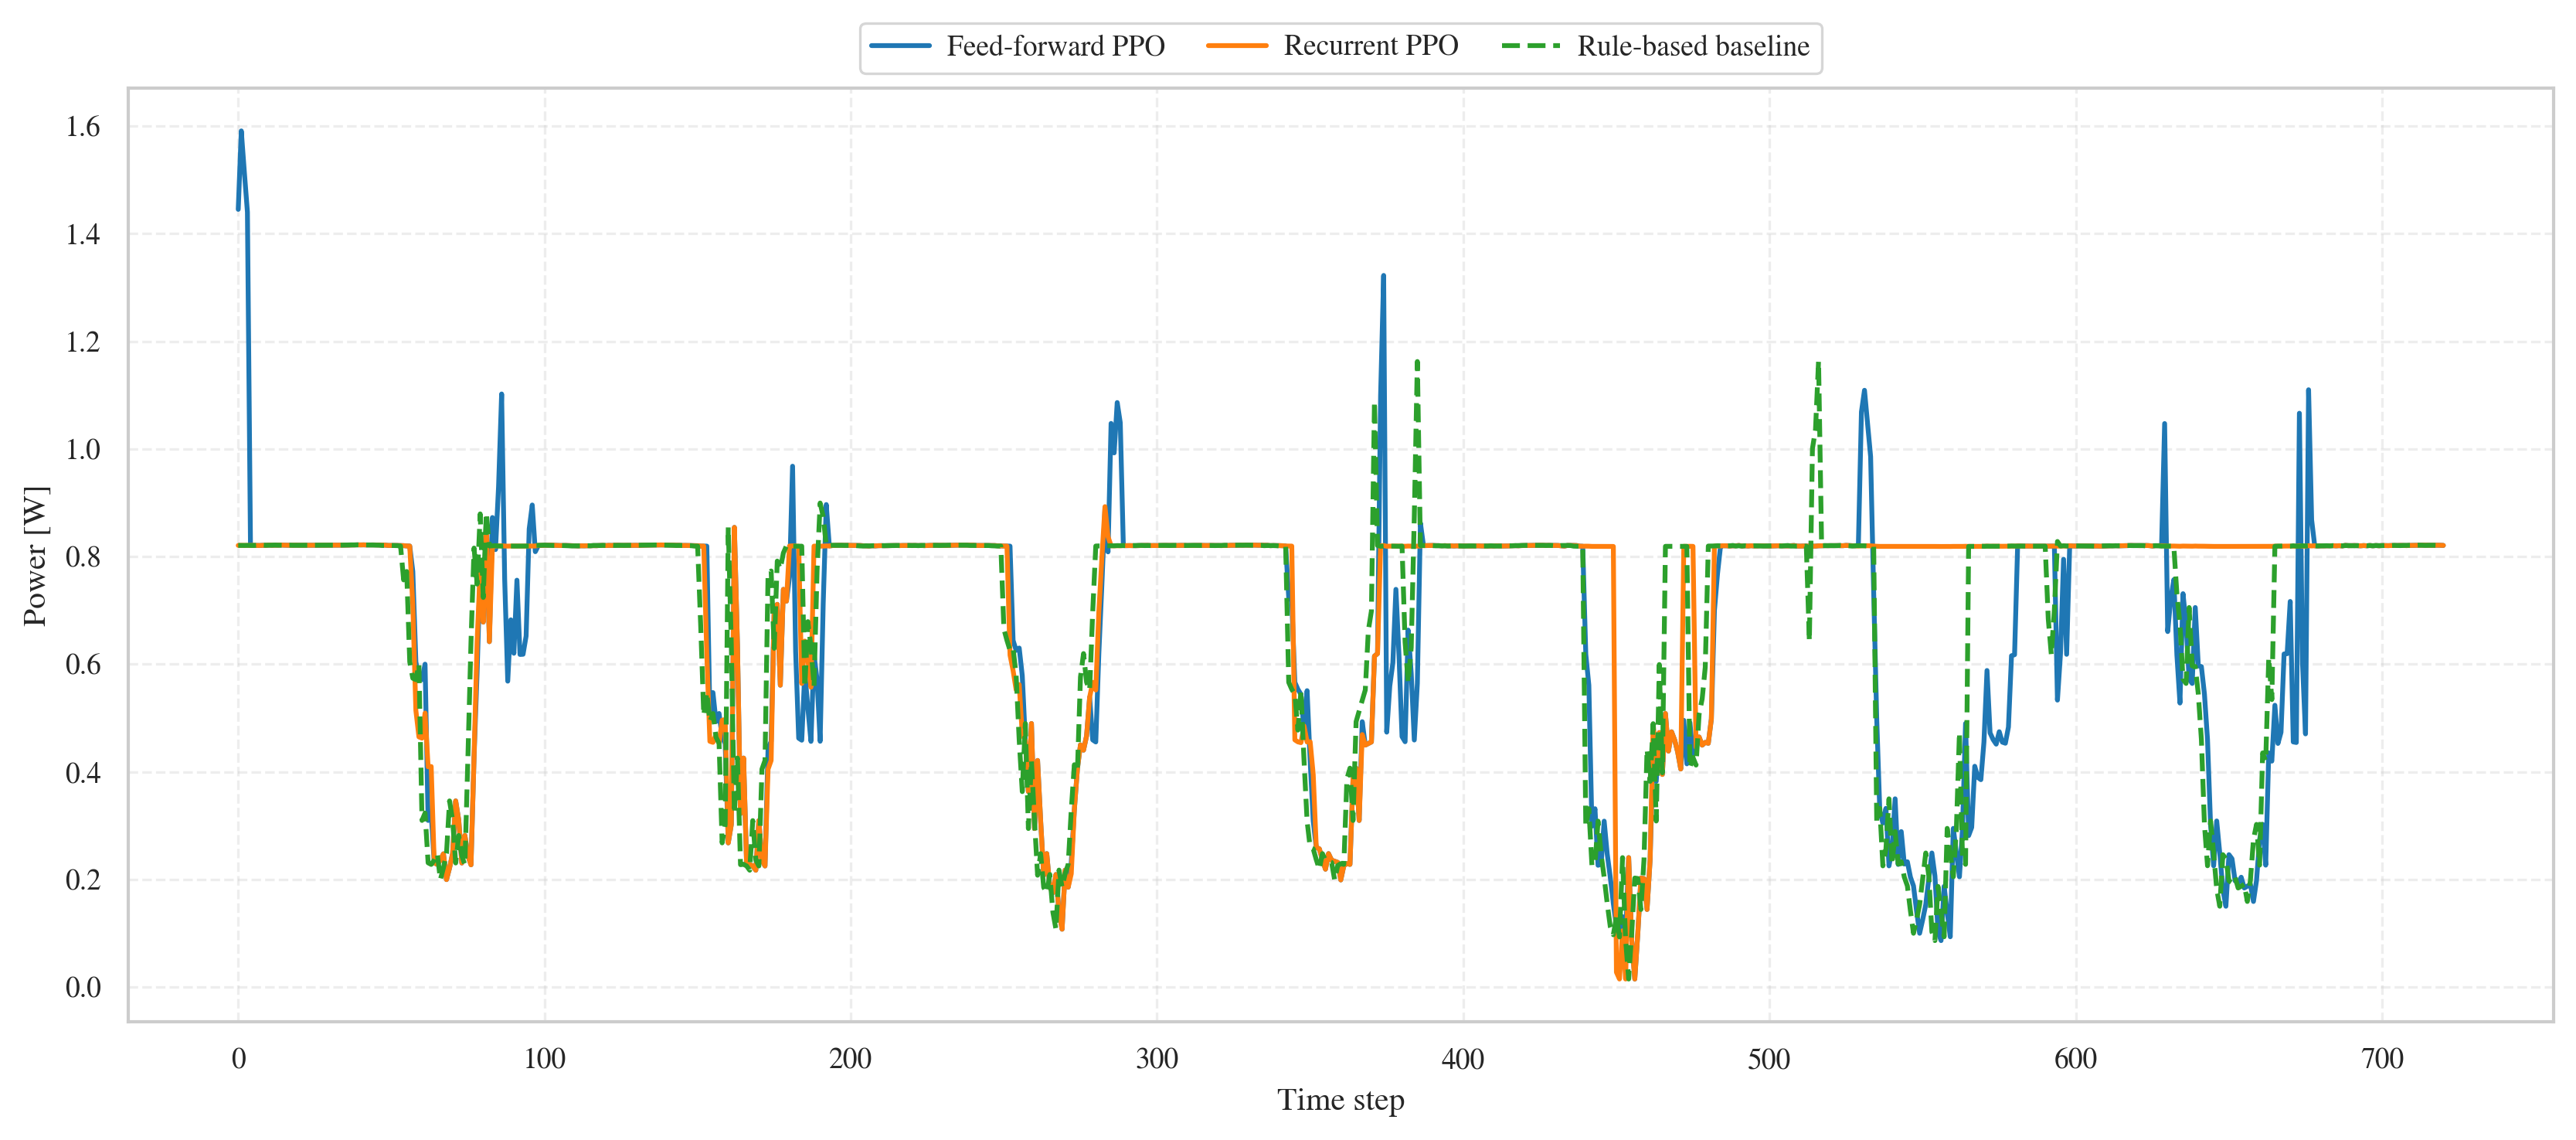
\includegraphics[width=.9\textwidth]{fig_power_timeline_locked_models.png}
\caption{Interval-averaged attributed power $P_t$ over the test horizon for the evaluated controllers.}
\label{fig:energy_time}
\end{figure}

To clarify where savings are realized, Figure~\ref{fig:sec_by_load} reports $\mathrm{SEC}_t$ aggregated by offered-load bins. The feed-forward PPO controller achieves its clearest advantage in the intermediate regime, where the trade-off between keeping DPDK active and scaling the user-space realization is most pronounced. The improvement relative to the rule-based baseline is also distributed broadly across the trace: over 51\% of time steps, the feed-forward PPO controller draws less attributed power than the rule-based controller. This suggests that the gain does not come from a single isolated regime.

\begin{figure}
\centering
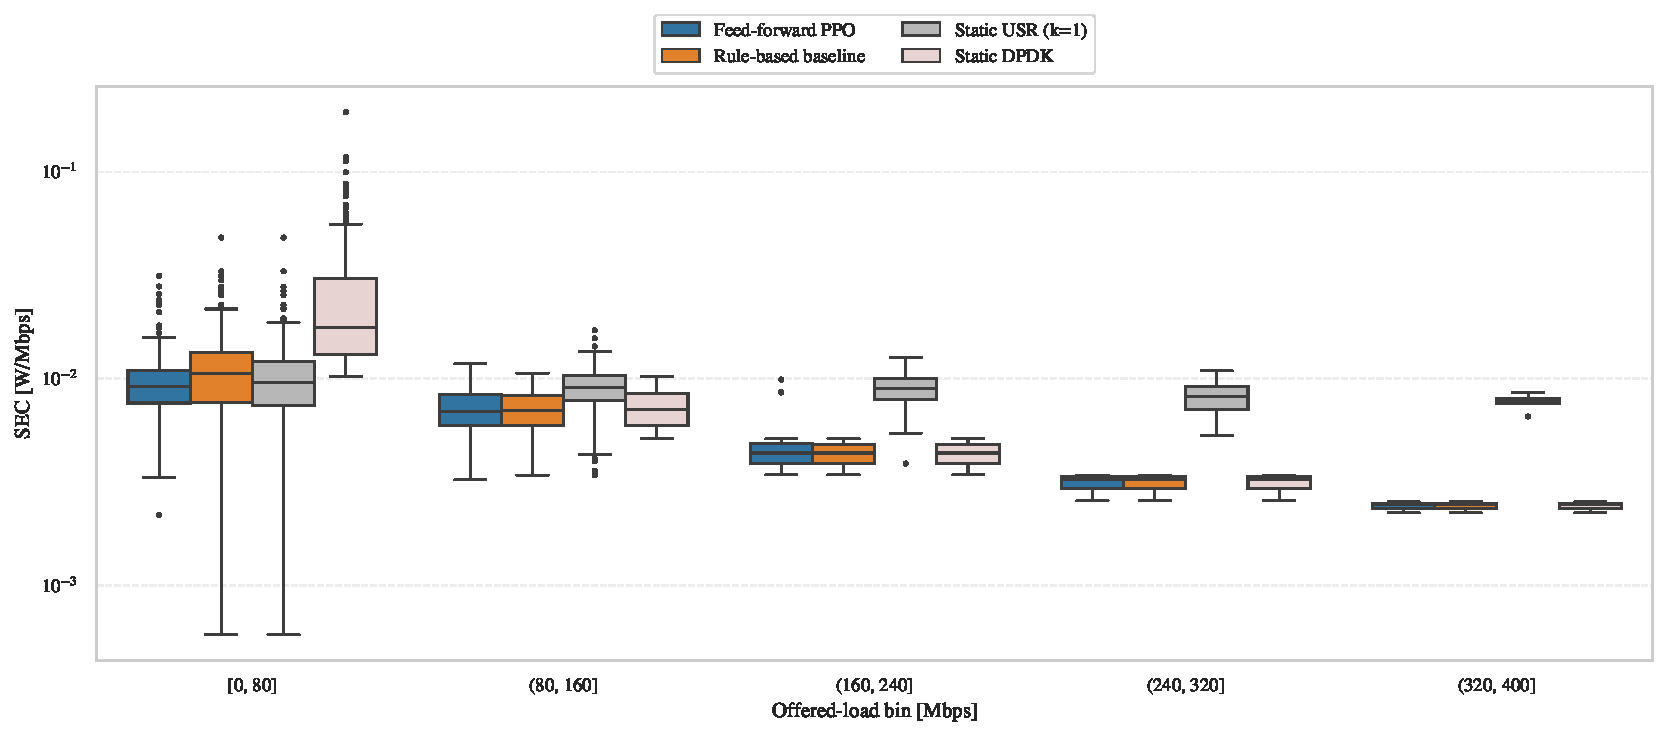
\includegraphics[width=.9\textwidth]{fig_sec_by_offered_load_bin_5models.pdf}
\caption{Specific energy consumption $\mathrm{SEC}_t$ by offered-load bins.}
\label{fig:sec_by_load}
\end{figure}

\subsection{QoS Compliance}
\label{subsec:qos_results}

QoS behavior is assessed through the compliance indicator $Q_t$ and the violation rate $v$ in~\eqref{eq:violation_rate}. Figure~\ref{fig:qos_time} shows the evolution of $Q_t$ over time and highlights intervals below the target $\tau$. Static user-space provisioning may violate the target during sustained high load when the fixed instance count becomes insufficient. Static DPDK generally improves compliance but at the cost of higher attributed energy over the full trace.

The feed-forward PPO controller maintains compliance by allocating sufficient capacity when traffic rises while avoiding persistent over-provisioning during low-load intervals. The violation rate reported in Table~\ref{tab:overall_results} confirms that the energy gains are not achieved by systematically trading off QoS. When violations occur, they tend to coincide with sharp load transitions or with intervals in which the cooldown guard delays an immediate reconfiguration.

\begin{figure}
\centering
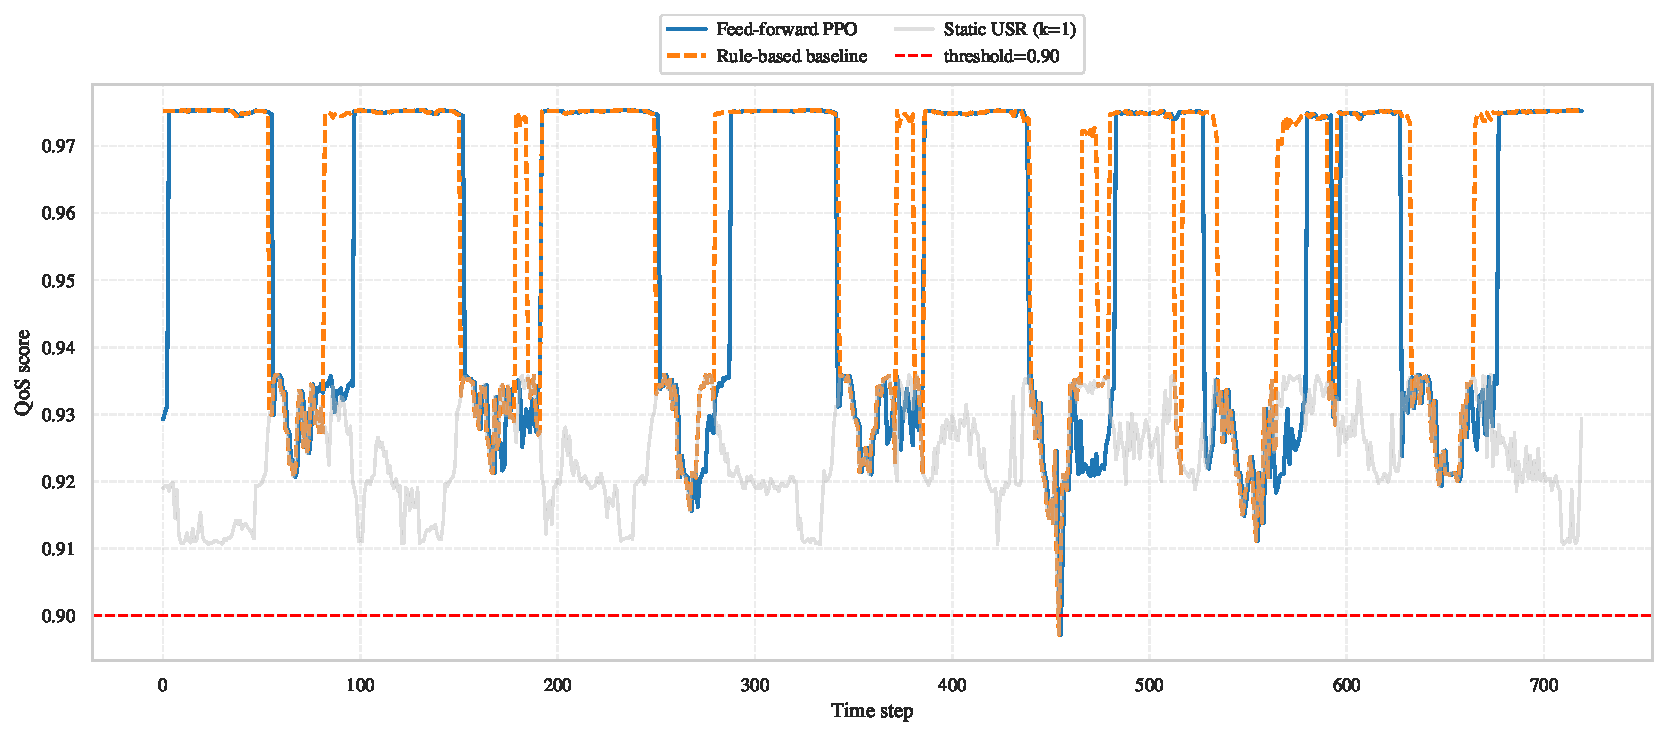
\includegraphics[width=.9\textwidth]{fig_qos_timeline_locked_models.pdf}
\caption{QoS-compliance indicator $Q_t$ over the test horizon. The dashed line marks the target $\tau$.}
\label{fig:qos_time}
\end{figure}

\subsection{Orchestration Behavior and Stability}
\label{subsec:stability_results}

Figure~\ref{fig:configs_time} reports the executed configuration sequence $\{c_t\}$ over time together with the offered load. The sequence illustrates how the learned policy partitions the load range into regions associated with different UPF modes and scale levels. Compared with the reactive heuristic, the feed-forward PPO controller produces stable actuation patterns with relatively long dwell times and limited oscillation around regime boundaries.

Table~\ref{tab:overall_results} disaggregates reconfigurations into type-switch events ($n_{\mathrm{sw}}$) and horizontal scaling events ($n_{\mathrm{sc}}$). This distinction is operationally relevant because a type switch is more disruptive than adding or removing a USR replica. The feed-forward PPO controller issues 17 type switches and 7 scaling events (24 total), while the rule-based baseline issues 24 type switches and no scaling events. The total number of actuations is therefore the same, but the learned controller substitutes some disruptive mode changes with lower-cost scaling operations. The recurrent PPO controller is the most conservative, issuing only 16 type switches and no scaling events, with 7 requests absorbed by the cooldown guard.

\begin{figure}
\centering
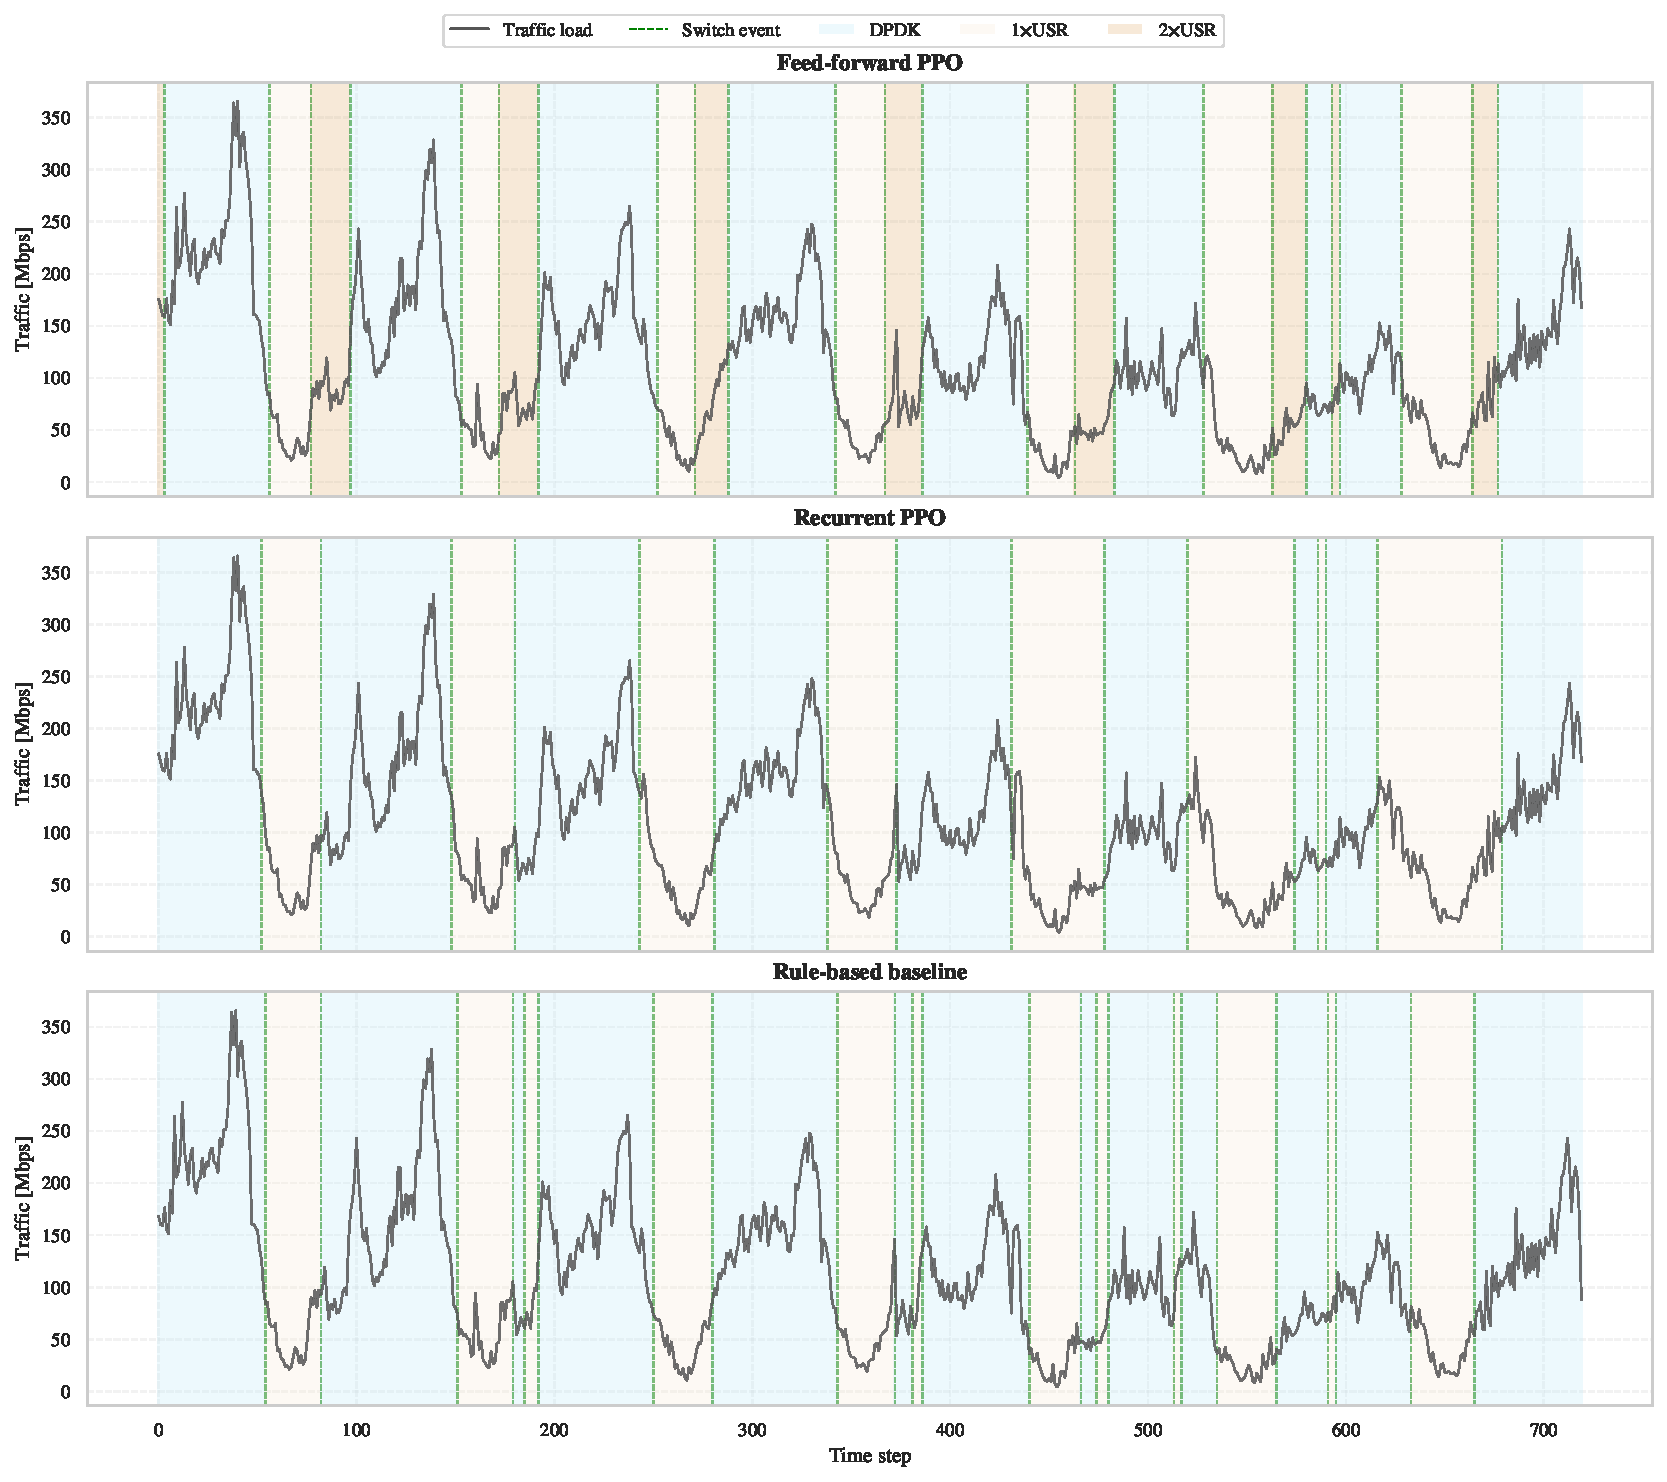
\includegraphics[width=\textwidth]{fig_configs_time_locked_models.pdf}
\caption{Executed configuration sequence $\{c_t\}$ over the test horizon.}
\label{fig:configs_time}
\end{figure}

\subsection{Ablation on Observation Schemas and Policy Parameterization}
\label{subsec:ablation_obs}

This subsection isolates the impact of temporal context in the observation and in the policy parameterization. We compare the instantaneous schema against history-augmented, forecast-augmented, and hybrid schemas, and we compare feed-forward PPO against recurrent PPO under matched training budgets.

Table~\ref{tab:ablation_obs} reports energy, QoS, and stability metrics for all considered combinations, disaggregated into type-switch ($n_{\mathrm{sw}}$) and scaling ($n_{\mathrm{sc}}$) events. For feed-forward PPO, only the hybrid schema activates horizontal scaling (7 scaling events), while all other schemas produce exclusively type switches. In our experiments, the combination of traffic history and forecast therefore provided the clearest context for exploiting the intermediate USR scaling level rather than oscillating between single-instance USR and DPDK. The instantaneous schema triggers the most type switches ($n_{\mathrm{sw}}=24$) despite comparable energy, indicating less stable actuation. The forecast-only schema is the most switch-conservative ($n_{\mathrm{sw}}=15$), but it yields slightly higher energy because it does not exploit scaling.

For recurrent PPO, the instantaneous and forecast-only schemas collapse to a fixed DPDK configuration ($n_{\mathrm{sw}}=0$, $E_{\mathrm{tot}}=147.79$~Wh), matching the static DPDK baseline. This suggests that, within the available training budget, those recurrent settings fail to learn a useful switching strategy. The history-augmented schema unlocks effective switching ($n_{\mathrm{sw}}=16$, $E_{\mathrm{tot}}=125.74$~Wh) with no scaling events, indicating a more conservative two-mode strategy. The hybrid recurrent schema produces only 4 type switches with no scaling, but occupies a weaker energy position ($E_{\mathrm{tot}}=132.38$~Wh). Overall, feed-forward PPO is more robust to schema choice and is the only controller that clearly exploits the full configuration space in the reported experiments.

\begin{table}[width=.9\linewidth,cols=6,pos=h]
\centering
\caption{Ablation results for observation schemas and policy parameterization. $n_{\mathrm{sw}}$ = type-switch events; $n_{\mathrm{sc}}$ = scaling events. Bold entries indicate the best result per policy variant. $\dagger$ denotes that the recurrent policy collapsed to a fixed configuration (no switching).}
\label{tab:ablation_obs}
\begin{tabular}{l l c c c c}
\hline
Policy & Observation schema & $E_{\mathrm{tot}}$ (Wh) & $v$ & $n_{\mathrm{sw}}$ & $n_{\mathrm{sc}}$ \\
\hline
PPO (feed-forward) & instantaneous    & 121.03 & 0.0014 & 24 & 0 \\
PPO (feed-forward) & history ($W$)    & 122.21 & 0.0014 & 19 & 0 \\
PPO (feed-forward) & forecast ($H$)   & 123.45 & 0.0014 & 15 & 0 \\
\textbf{PPO (feed-forward)} & \textbf{hybrid} & \textbf{120.79} & \textbf{0.0014} & \textbf{17} & \textbf{7} \\
\hline
PPO (recurrent) & instantaneous       & 147.79 & 0.0000 & $0^\dagger$ & 0 \\
PPO (recurrent) & forecast ($H$)      & 147.79 & 0.0000 & $0^\dagger$ & 0 \\
\textbf{PPO (recurrent)} & \textbf{history ($W$)} & \textbf{125.74} & \textbf{0.0014} & \textbf{16} & \textbf{0} \\
PPO (recurrent) & hybrid              & 132.38 & 0.0042 & 4 & 0 \\
\hline
\end{tabular}
\end{table}

\subsection{Sensitivity Analysis}
\label{subsec:sensitivity}

This subsection examines the sensitivity of the feed-forward PPO controller to three design parameters: the cooldown length $I_c$, the QoS compliance target $\tau$, and the maximum number of admissible user-space instances $k_{\max}$.

\subsubsection{Cooldown Length $I_c$}
\label{subsubsec:sensitivity_ic}

We analyze sensitivity to the cooldown length $I_c$ using the feed-forward PPO controller with the hybrid observation schema. With $I_c=0$ (no cooldown), the controller produces 36 reconfigurations and a violation rate of $v=0.0097$, indicating that unrestricted actuation leads to oscillatory behavior that degrades QoS. Increasing the cooldown to $I_c=2$ already suppresses most oscillations ($n_{\mathrm{reconf}}=17$, $v=0.0014$) with only a marginal energy penalty. The default setting $I_c=4$ maintains the same violation rate and reconfiguration count while achieving the lowest total attributed energy at 120.80~Wh. Further increasing to $I_c=8$ slightly raises energy (121.55~Wh) and violation rate ($v=0.0042$), as the extended lockout prevents timely adaptation to rapid load changes. These results suggest that the chosen cooldown of $I_c=4$ is a reasonable operating point for this testbed-derived setting.

\subsubsection{QoS Compliance Target $\tau$}
\label{subsubsec:sensitivity_tau}

The QoS-compliance target $\tau$ controls the threshold below which the reward penalty is applied and directly shapes how conservatively the agent selects configurations. Figure~\ref{fig:sensitivity_tau} reports the effect of varying $\tau \in \{0.90, 0.95\}$ on the DPDK utilization share and QoS violation rate for both PPO variants.

At $\tau=0.95$, the feed-forward PPO controller allocates DPDK in 71.4\% of time steps, a shift of $+15.8$ percentage points relative to the $\tau=0.90$ operating point (55.6\%). The recurrent variant exhibits a similar shift, increasing its DPDK share from 61.3\% to 74.7\% ($+13.4$~pp). Despite this more conservative behavior, the violation rate rises sharply to $v=0.20$--$0.37$ for both variants, indicating that the available USR configurations cannot consistently satisfy the stricter target under this workload. The number of reconfigurations also drops at $\tau=0.95$, as the agents remain in DPDK more often. In this setting, $\tau=0.90$ is therefore better matched to the QoS capabilities of the current profiled configurations.

\begin{figure}
\centering
\begin{subfigure}[!t]{0.48\textwidth}
  \centering
  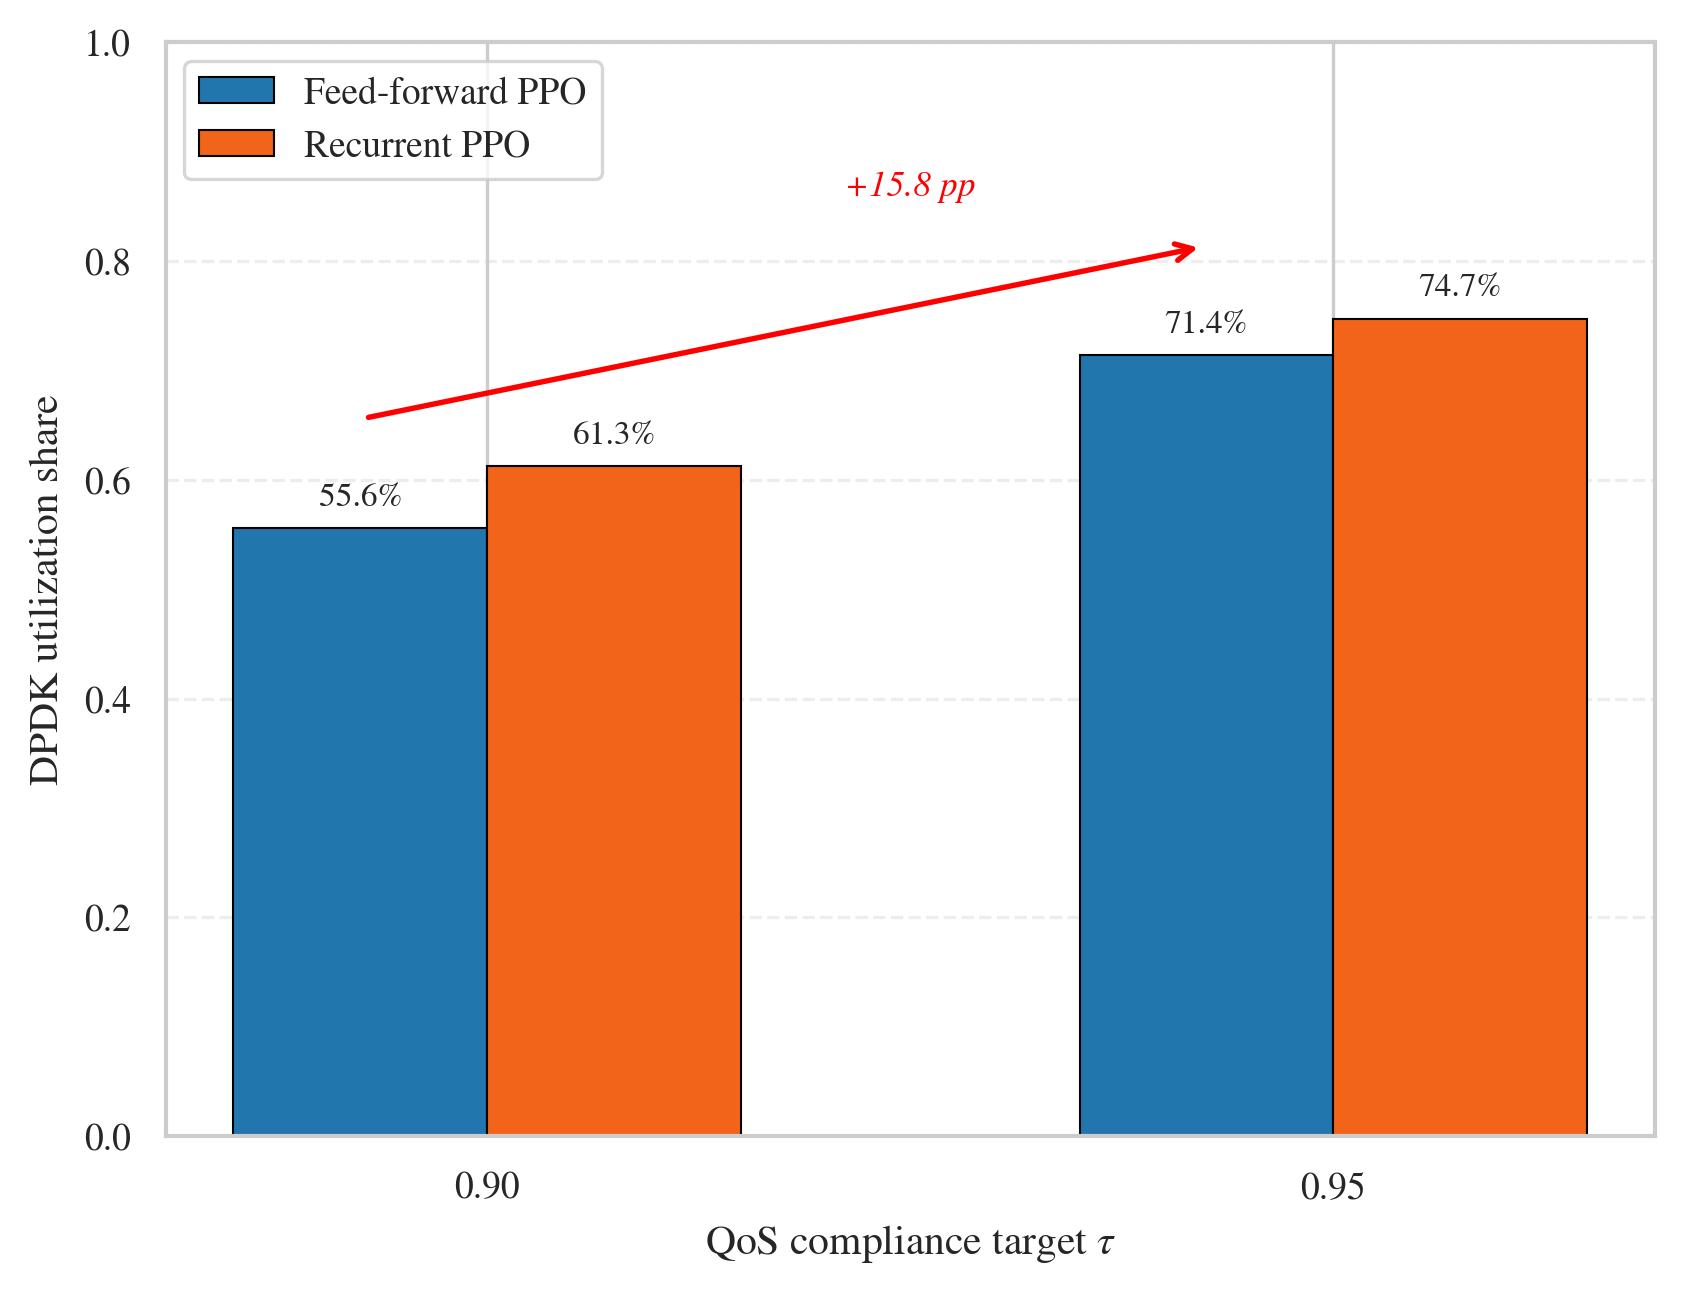
\includegraphics[width=.9\textwidth]{fig_threshold_dpdk_stickiness.png}
  \caption{DPDK utilization share.}
  \label{fig:sensitivity_tau_dpdk}
\end{subfigure}
\hfill
\begin{subfigure}[!t]{0.48\textwidth}
  \centering
  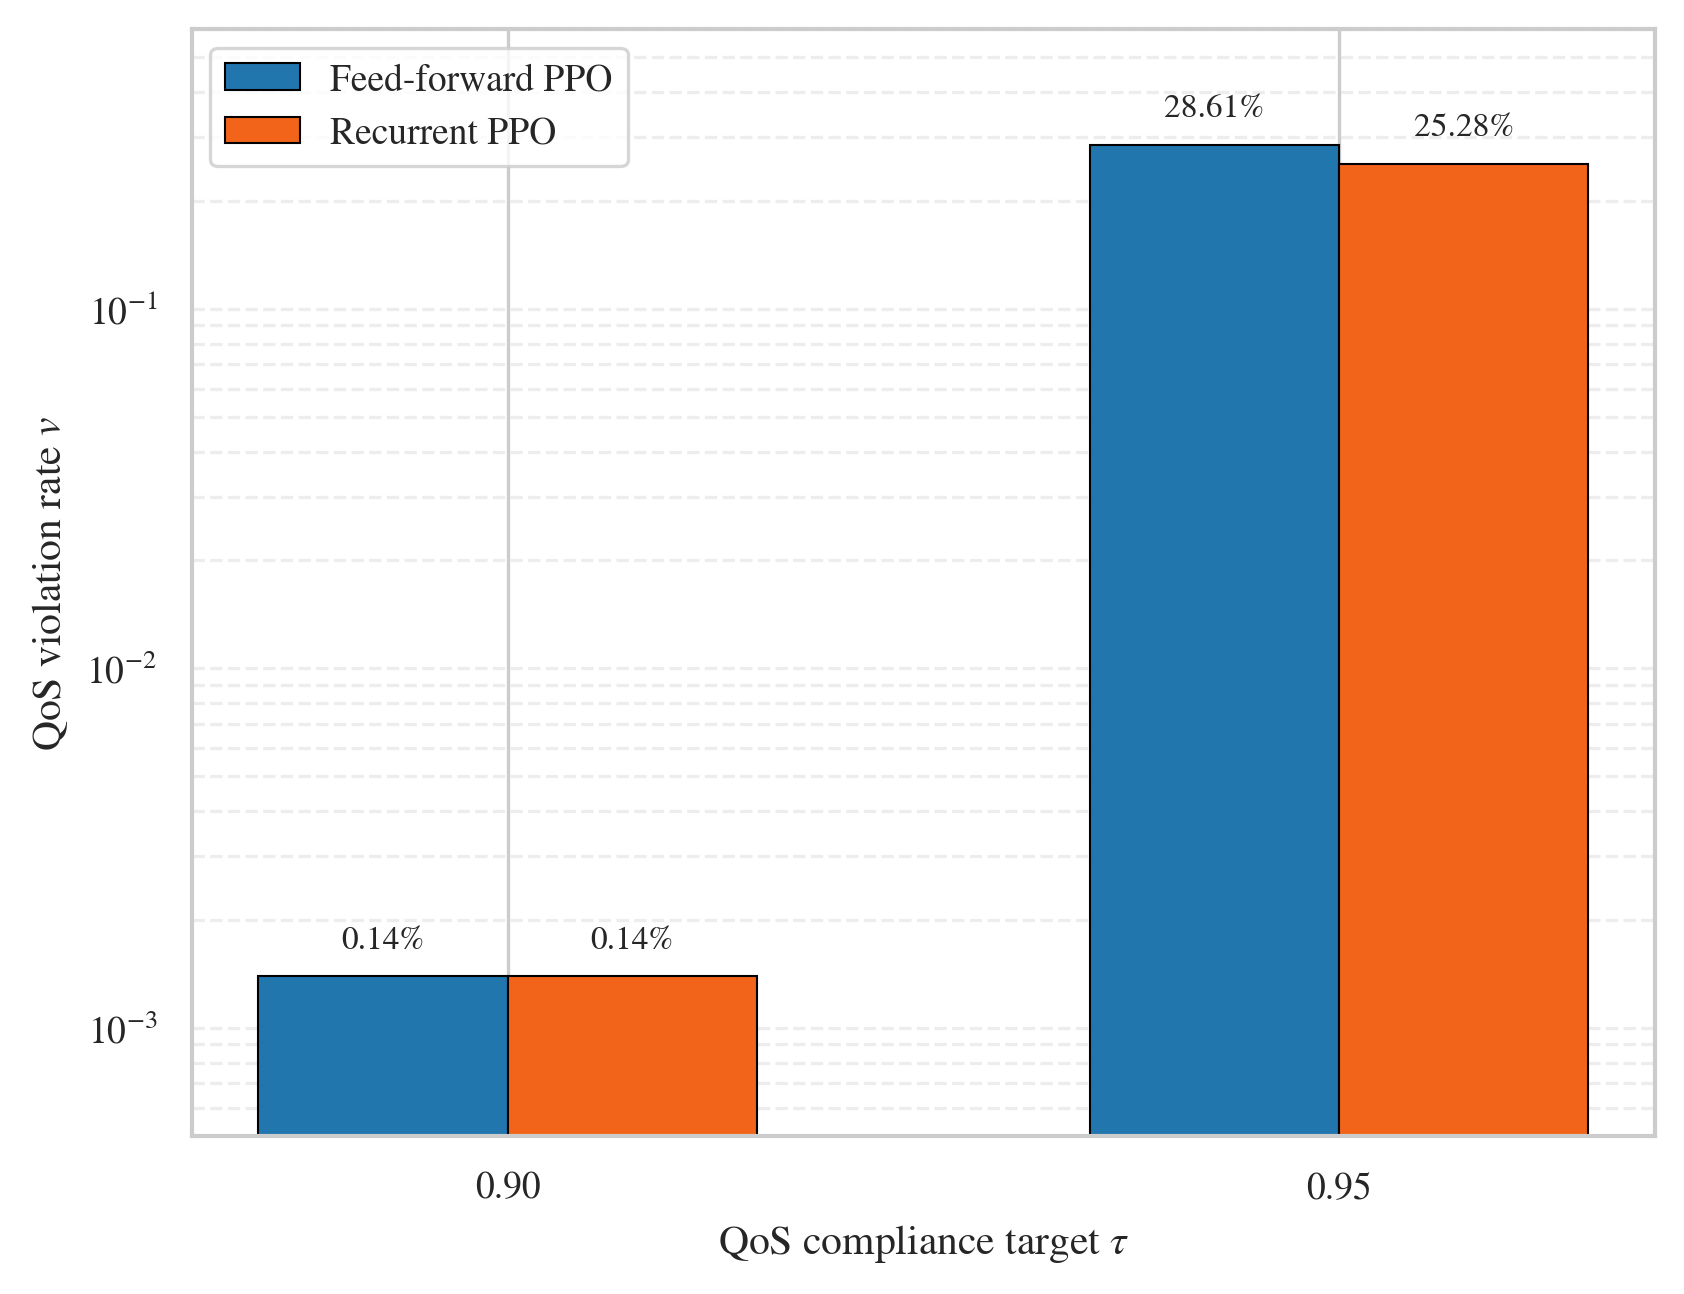
\includegraphics[width=.9\textwidth]{fig_threshold_violation_rate.png}
  \caption{QoS violation rate.}
  \label{fig:sensitivity_tau_viol}
\end{subfigure}
\caption{Effect of QoS-compliance target $\tau$ on DPDK utilization share and QoS violation rate for feed-forward and recurrent PPO.}
\label{fig:sensitivity_tau}
\end{figure}

\subsubsection{Maximum User-Space Instance Count $k_{\max}$}
\label{subsubsec:sensitivity_k}

The maximum number of admissible user-space instances $k_{\max}$ determines the scaling headroom available to the agent. Table~\ref{tab:sensitivity_k} reports the effect of restricting $k_{\max} \in \{1,2\}$ at $\tau=0.90$ for both PPO variants.

\begin{table}[width=.9\linewidth,cols=5,pos=h]
\centering
\caption{Effect of maximum instance count $k_{\max}$ on energy and stability at $\tau=0.90$.}
\label{tab:sensitivity_k}
\begin{tabular}{l c c c c}
\hline
Policy & $k_{\max}$ & $E_{\mathrm{tot}}$ (Wh) & $v$ & $n_{\mathrm{reconf}}$ \\
\hline
PPO (feed-forward) & 1 & 123.32 & 0.0014 & 20 \\
PPO (feed-forward) & 2 & 120.80 & 0.0014 & 17 \\
PPO (recurrent)    & 1 & 121.80 & 0.0014 & 14 \\
PPO (recurrent)    & 2 & 125.74 & 0.0014 & 16 \\
\hline
\end{tabular}
\end{table}

The feed-forward PPO controller benefits from the larger configuration space: expanding from $k_{\max}=1$ to $k_{\max}=2$ reduces total attributed energy by 2.0\% (from 123.32 to 120.80~Wh) and reduces the reconfiguration count from 20 to 17, because the two-instance USR level provides an intermediate option for moderate-to-high loads. In contrast, the recurrent PPO variant achieves its lowest energy (121.80~Wh) and fewest reconfigurations (14) at $k_{\max}=1$, suggesting that it does not effectively exploit the additional scaling level within the available training budget.

\subsection{Seed Robustness}
\label{subsec:seed_robustness}

To assess training stability, we evaluate both PPO variants across five independently seeded training runs using fixed hyperparameters and identical evaluation conditions. Since the main comparison reports mean $\pm$ standard deviation across seeds, Table~\ref{tab:seed_robustness} is retained as a detailed per-seed breakdown that exposes the spread and the main outliers behind those aggregate values.

\begin{table}[width=.9\linewidth,cols=5,pos=h]
\centering
\caption{Per-seed results for feed-forward and recurrent PPO across five training seeds on the main held-out evaluation split.}
\label{tab:seed_robustness}
\begin{tabular}{l c c c c}
\hline
Policy & Seed & $E_{\mathrm{tot}}$ (Wh) & $v$ & $n_{\mathrm{reconf}}$ \\
\hline
PPO (feed-forward) & 42   & 122.94 & 0.0028 & 18 \\
PPO (feed-forward) & 123  & 122.33 & 0.0014 & 14 \\
\textbf{PPO (feed-forward)} & \textbf{456}  & \textbf{120.79} & \textbf{0.0014} & \textbf{17} \\
PPO (feed-forward) & 789  & 121.98 & 0.0097 & 20 \\
PPO (feed-forward) & 1024 & 124.88 & 0.0014 & 24 \\
\hline
PPO (recurrent)    & 42   & 122.11 & 0.0083 & 38 \\
PPO (recurrent)    & 123  & 134.01 & 0.0014 & 18 \\
\textbf{PPO (recurrent)} & \textbf{456}  & \textbf{125.74} & \textbf{0.0014} & \textbf{16} \\
PPO (recurrent)    & 789  & 122.72 & 0.0097 & 14 \\
PPO (recurrent)    & 1024 & 121.92 & 0.0097 & 14 \\
\hline
\end{tabular}
\end{table}

The feed-forward PPO controller exhibits relatively tight seed-to-seed variation, with total attributed energy ranging from 120.79 to 124.88~Wh and an aggregate result of $122.58 \pm 1.50$~Wh. Its average SEC is likewise stable at $0.00748 \pm 0.00015$~Wh/Mbit, and its mean violation rate remains low at $0.00333 \pm 0.00362$. The recurrent PPO controller shows much wider variation, from 121.92 to 134.01~Wh, with a substantially broader aggregate spread of $125.29 \pm 5.11$~Wh and $0.00804 \pm 0.00124$~Wh/Mbit in average SEC. It also exhibits stronger behavioral variability, including a high-switching outlier (seed~42) and substantially more blocked requests on average. These results confirm that the feed-forward controller is the more reliable choice for this setting.

\subsection{Cross-Trace Generalization}
\label{subsec:generalization}

The results presented so far are obtained on the Main trace, which is also the trace used for training. To assess whether the learned policies generalize to an unseen traffic profile, we evaluate all controllers on the YouTube trace described in Section~\ref{subsec:workload}. The PPO policies are not retrained; the same five-seed checkpoints trained on the Main trace are replayed on the YouTube workload through the same digital twin.

Table~\ref{tab:overall_results_youtube} reports the results. The static baselines confirm that the YouTube trace exercises a different load distribution: Static~USR($k=1$) consumes less energy (165.33~Wh vs.\ 178.76~Wh on Main), and the rule-based baseline achieves zero QoS violations, indicating that the YouTube load stays further from the USR saturation boundary.

\begin{table}[width=.9\linewidth,cols=7,pos=h]
\centering
\caption{Overall results on the YouTube trace (cross-trace generalization). The PPO policies are identical to those trained on the Main trace and are not retrained. Notation follows Table~\ref{tab:overall_results}.}
\label{tab:overall_results_youtube}
\small
\resizebox{\columnwidth}{!}{%
\begin{tabular}{l c c c c c c}
\hline
Controller & $E_{\mathrm{tot}}$ & $\overline{\mathrm{SEC}}$ & $v$ & $n_{\mathrm{sw}}$ & $n_{\mathrm{sc}}$ & $n_{\mathrm{bl}}$ \\
\hline
Offline-optimal reference    & 116.70          & 0.00698          & 0.0166          & 31 & 18 & 0 \\
\textbf{PPO (feed-forward)} & \textbf{124.47 $\pm$ 1.60} & \textbf{0.00782 $\pm$ 0.00025} & \textbf{0.00442 $\pm$ 0.00721} & 16.4 $\pm$ 3.5 & 10.8 $\pm$ 6.8 & 14.8 $\pm$ 13.7 \\
PPO (recurrent)             & 126.77 $\pm$ 5.74          & 0.00868 $\pm$ 0.00230          & 0.00996 $\pm$ 0.00909 & 20.4 $\pm$ 13.0 & 4.4 $\pm$ 3.2 & 25.6 $\pm$ 25.6 \\
Rule-based baseline         & 123.57          & 0.00797          & 0.0000          & 16 & 0 & 1 \\
Static DPDK                 & 147.78          & 0.01521          & 0.0000          & - & - & - \\
Static USR($k=1$)           & 165.33          & 0.00917          & 0.0000          & - & - & - \\
\hline
\end{tabular}
}
\end{table}

The feed-forward PPO controller reduces mean total attributed energy by 15.8\% relative to Static~DPDK on the YouTube trace ($124.47$ vs.\ $147.78$~Wh), which is comparable to the 16.9\% reduction observed on the Main trace. However, its margin over the rule-based baseline narrows: mean energy is slightly higher ($+0.73\%$), while mean SEC remains lower ($0.00782$ vs.\ $0.00797$~Wh/Mbit, $-1.9\%$). This narrower margin is expected because the YouTube trace is less demanding and the rule-based controller already achieves zero violations, leaving less room for an adaptive policy to exploit intermediate configurations.

The feed-forward PPO controller continues to outperform the recurrent variant on YouTube, with lower mean energy ($-1.8\%$), lower mean SEC ($-9.9\%$), and lower mean violation rate. The recurrent variant also exhibits wider seed-to-seed variation, with one outlier seed (seed~123) reaching $136.38$~Wh. These patterns are consistent with the Main-trace findings and confirm that the relative ranking of the two PPO parameterizations is preserved across workloads.

Overall, the feed-forward PPO controller demonstrates that the energy-efficiency gains over static provisioning are robust to workload change, while the margin over the engineered rule-based baseline is workload-dependent and narrows on a less demanding trace.

\subsection{Statistical Significance Analysis}
\label{subsec:stat_significance}

The multi-seed evaluation in Section~\ref{subsec:seed_robustness} reports mean and standard deviation across five independently trained seeds. To assess whether the observed differences are statistically robust, we apply the Wilcoxon signed-rank test~\cite{wilcoxon1945individual} to the paired per-seed outcomes on the Main trace. This non-parametric test is appropriate for small paired samples and does not assume normality.

We test the central comparison of the paper: feed-forward PPO versus the rule-based baseline. For each of the five seeds, we compute the paired difference in total energy $E_{\mathrm{tot}}$, mean SEC $\overline{\mathrm{SEC}}$, and QoS violation rate $v$. The null hypothesis is that the median paired difference is zero (two-tailed).

Table~\ref{tab:wilcoxon} reports the test statistics. With $n=5$ paired observations, the minimum achievable $p$-value for the Wilcoxon signed-rank test is $p=0.0625$, which cannot reach the conventional $\alpha=0.05$ significance level regardless of how consistent the results are. This is a structural consequence of the sample size rather than an indication of weak effects.

\begin{table}[width=.9\linewidth,cols=5,pos=h]
\centering
\caption{Wilcoxon signed-rank test results for feed-forward PPO vs.\ rule-based baseline on the Main trace. $n_{\mathrm{better}}$: seeds where FF-PPO improves over the baseline; $W$: test statistic; $p$: two-tailed $p$-value. The minimum achievable $p$ with $n=5$ is 0.0625.}
\label{tab:wilcoxon}
\begin{tabular}{l c c c c}
\hline
Metric & $n_{\mathrm{better}}$ / $n$ & $\Delta$ mean & $W$ & $p$ \\
\hline
$E_{\mathrm{tot}}$ (Wh)             & 4/5 & $-1.74$ ($-1.40\%$) & 1.0 & 0.1250 \\
$\overline{\mathrm{SEC}}$ (Wh/Mbit) & 5/5 & $-0.00030$ ($-3.86\%$) & 0.0 & 0.0625 \\
$v$                                  & 0/5 & $+0.00194$           & 0.0 & 0.5000 \\
\hline
\end{tabular}
\end{table}

The SEC comparison yields $W=0.0$ and $p=0.0625$: all five seeds achieve lower SEC than the rule-based baseline, and the test statistic reaches the minimum achievable $p$-value. This is the strongest possible result obtainable with five paired samples. The total energy comparison yields $p=0.1250$, with four of five seeds improving over the baseline. The QoS violation rate shows no significant difference ($p=0.5000$), consistent with the design intent that the PPO controller should match, not necessarily improve, the baseline's QoS behavior.

Figure~\ref{fig:wilcoxon_main} visualizes the paired per-seed differences and the Wilcoxon test outcome for the feed-forward PPO versus rule-based comparison.

\begin{figure}
\centering
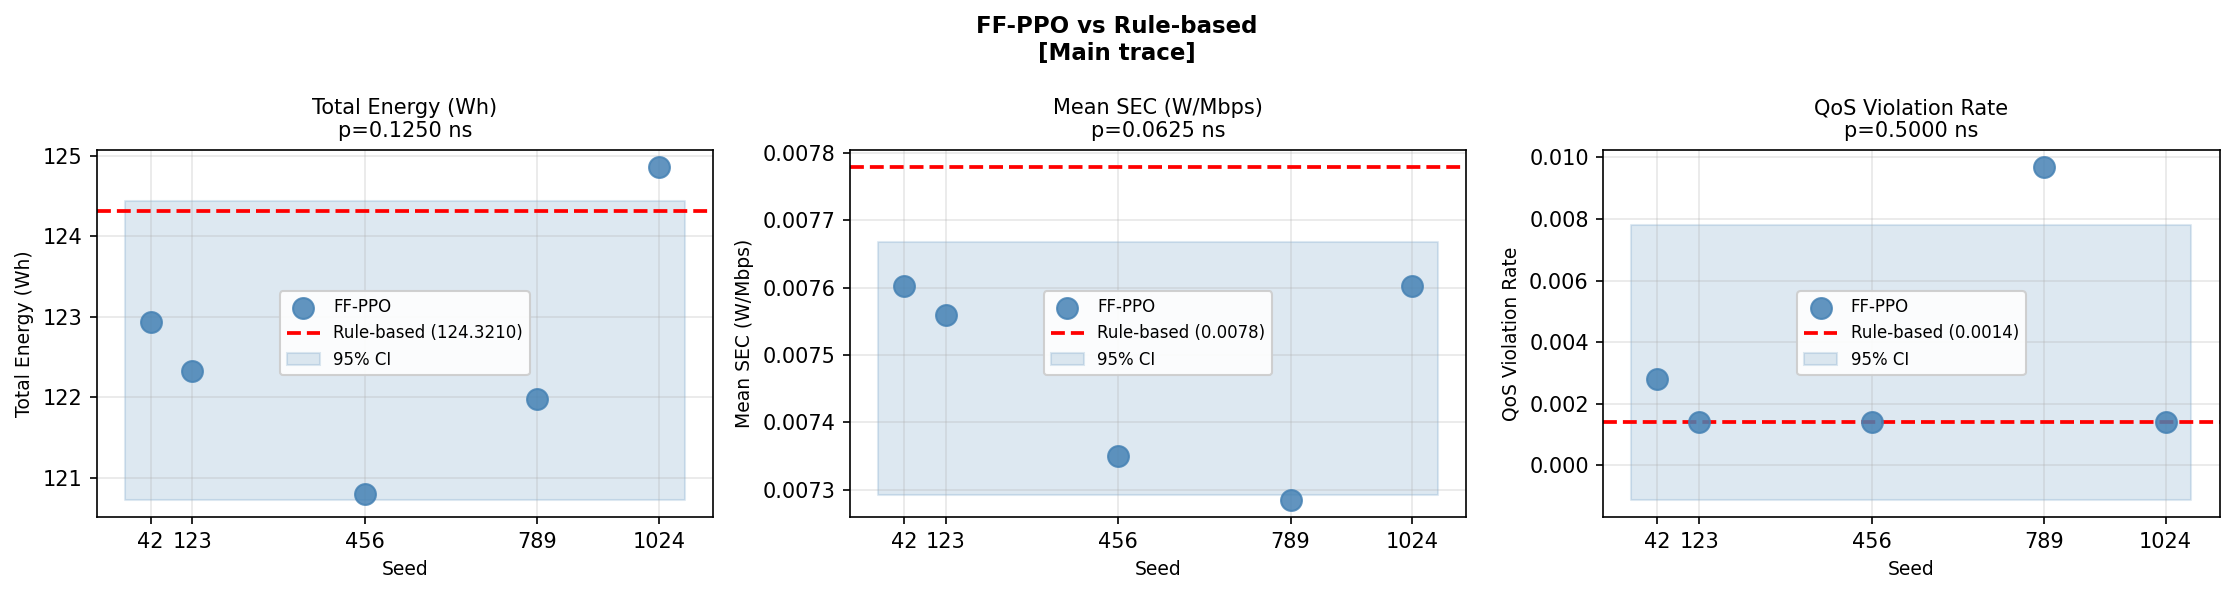
\includegraphics[width=.9\textwidth]{plot_mlp_vs_rule_main.png}
\caption{Wilcoxon signed-rank test visualization for feed-forward PPO vs.\ rule-based baseline on the Main trace. Each point represents one training seed; the dashed line marks zero difference.}
\label{fig:wilcoxon_main}
\end{figure}

These results confirm that the SEC improvement is consistent across all five seeds, and the inability to reach $\alpha=0.05$ is a limitation of the sample size rather than of the effect magnitude. Increasing the number of independently trained seeds in future work would allow conventional significance testing.

\subsection{Summary of Findings}
\label{subsec:results_summary}

The feed-forward PPO controller with the hybrid observation schema is the strongest causal controller in the reported setting. Its key advantage over the rule-based baseline is not a large energy margin but a qualitative difference in actuation strategy: it combines fewer type switches with effective use of horizontal scaling, replacing some disruptive mode changes with lower-cost scaling actions. Relative to the offline-optimal reference, it closes a larger share of the remaining performance gap than the rule-based controller, even though the exact planner operates with full future knowledge. The ablation study shows that this behavior emerges only with the hybrid observation schema, and the multi-seed analysis confirms that feed-forward PPO is more robust than recurrent PPO under the available training budget.

Cross-trace evaluation on the YouTube workload confirms that the energy-efficiency gains over static provisioning are preserved (15.8\% reduction vs.\ Static~DPDK), while the margin over the rule-based baseline is workload-dependent and narrows on a less demanding trace. Wilcoxon signed-rank tests on the Main trace show that the SEC improvement over the rule-based baseline is consistent across all five seeds, reaching the minimum achievable $p$-value ($p=0.0625$) for the available sample size.


\section{Conclusion}
\label{conclusion}

This paper presented an AI-driven framework for energy-aware orchestration of User Plane Functions in 5G Core networks. The framework models UPF orchestration as a constrained sequential decision problem with an explicit cooldown guard, asymmetric reconfiguration costs, and a multi-objective reward balancing energy efficiency, QoS compliance, and actuation stability. A Proximal Policy Optimization controller is trained and evaluated in a measurement-grounded digital twin constructed from profiling data collected on a physical testbed.

On the main held-out evaluation split, the feed-forward PPO controller remains the strongest causal controller across five seeds, achieving $122.58 \pm 1.50$~Wh total attributed energy and $0.00748 \pm 0.00015$~Wh/Mbit average SEC. This corresponds to roughly a 16.9\% reduction in mean total attributed energy relative to static DPDK provisioning and a more modest 1.1\% reduction relative to the deterministic rule-based threshold baseline, while preserving a low mean QoS violation rate of $0.00333 \pm 0.00362$. Relative to a non-causal offline-optimal reference computed by exact planning under the same discounted reward objective and cooldown constraints, the mean feed-forward PPO controller remains 5.48\% above the attainable optimum in the deterministic twin, whereas the rule-based baseline remains 6.64\% above it. The learned policy achieves its improvement by dynamically choosing between a DPDK-based and a cloud-native UPF realization and, in the best-performing observation setting, exploiting horizontal scaling to replace some disruptive mode switches with lower-cost scaling actions.

Cross-trace generalization was validated on a second, independently derived YouTube-based workload. Without retraining, the feed-forward PPO controller reduces mean total attributed energy by 15.8\% relative to static DPDK provisioning on the YouTube trace, confirming that the energy-efficiency gains are preserved across workloads. The margin over the rule-based baseline is workload-dependent and narrows on the less demanding YouTube trace, where the rule-based controller already achieves zero QoS violations. Wilcoxon signed-rank tests on the Main trace confirm that the SEC improvement over the rule-based baseline is consistent across all five seeds, reaching the minimum achievable $p$-value ($p=0.0625$) for the available sample size.

These results support the use of constraint-aware reinforcement learning for improving the energy--QoS--stability trade-off in a measurement-grounded 5GC user-plane setting under offline digital-twin validation. More broadly, the framework's modular integration of analytics functions (NWDAF, MDAF) with a learning-based decision module provides a template for intelligence-driven orchestration of other network functions in next-generation mobile networks. Future work will extend the framework to larger configuration spaces, an increased number of training seeds to strengthen statistical conclusions, stochastic digital twins, and live closed-loop validation.


% ===========================================================================
% APPENDIX
% ===========================================================================

\appendix
\section{Notation Reference}
\label{app:notation}

Table~\ref{tab:notation} summarizes the main symbols used throughout the paper.

\begin{table}[width=.9\linewidth,cols=2,pos=h]
\centering
\caption{Summary of notation.}
\label{tab:notation}
\small
\begin{tabular}{l l}
\hline
Symbol & Description \\
\hline
$\mathcal{M}$ & Set of UPF realization modes \\
$\mathcal{K}_m$ & Admissible instance counts for mode $m$ \\
$c_t=(m_t,k_t)$ & Executed configuration at slot $t$ \\
$\mathcal{C}$ & Configuration space \\
$a_t$ & Configuration command issued by the agent \\
$\Delta$ & Control period (slot duration) \\
$x_t$ & Observation vector at slot $t$ \\
$\rho_t$ & Offered load at slot $t$ \\
$P_t$ & Interval-averaged UPF-attributed power \\
$Q_t$ & Scalar QoS-compliance score \\
$E_{\mathrm{tot}}$ & Total attributed energy over the evaluation \\
$\mathrm{SEC}_t$ & Specific energy consumption at slot $t$ \\
$u_t$ & Cooldown counter (slots since last reconfiguration) \\
$I_c$ & Cooldown length (in slots) \\
$\tau$ & QoS-compliance target threshold \\
$v$ & QoS violation rate \\
$\pi_\theta$ & Parameterized policy \\
$r_t$ & Reward at slot $t$ \\
$\gamma$ & Discount factor \\
$\alpha$ & SEC scaling weight in reward \\
$\lambda_{\mathrm{QoS}}$ & QoS penalty weight in reward \\
$\mathcal{T}(\cdot)$ & Digital-twin transition function \\
$p_m(\rho),\,q_m(\rho)$ & Profiling models for power and QoS \\
$n_{\mathrm{sw}}$ & Number of type-switch events \\
$n_{\mathrm{sc}}$ & Number of horizontal scaling events \\
$n_{\mathrm{bl}}$ & Number of cooldown-blocked requests \\
\hline
\end{tabular}
\end{table}


% ===========================================================================
% END MATTER
% ===========================================================================

% CRediT author contributions (printed automatically from \credit{} above)
\printcredits

% \section*{Data availability}
% The evaluation workload is derived from the publicly available NetMob 2023 dataset. Code and trained models will be made available upon reasonable request.
\section*{Acknowledgements}
This work was supported in part by the European Union's Horizon Europe programme under the SUNRISE-6G project (Grant Agreement No.\ 101139075) and in part by the European Union under the Italian National Recovery and Resilience Plan (NRRP) of NextGenerationEU, Mission 4, Component 2, Investment 1.3, CUP F83C22001690001, partnership on ``Telecommunications of the Future'' (PE00000001 -- program ``RESTART'').

%\section*{Acknowledgements}
% Add funding acknowledgements here if applicable.

%% Loading bibliography style file
\bibliographystyle{cas-model2-names}

% Loading bibliography database
\bibliography{references}

\end{document}